
\documentclass[11pt]{article}

\usepackage[utf8]{inputenc}
\usepackage[T1]{fontenc}
\usepackage{lmodern}
\usepackage{microtype}
\usepackage[margin=1in]{geometry}
\usepackage{biocon}
\usepackage{amsmath}
\usepackage{amssymb}
\usepackage{graphicx}
\usepackage{xcolor}
\usepackage{hyperref}
\usepackage{cleveref}
\usepackage{natbib}

\graphicspath{{images/}}

\hypersetup{
  colorlinks=true,
  linkcolor=blue!50!black,
  citecolor=blue!50!black,
  urlcolor=blue!50!black,
}


% notation


\graphicspath{{images/}} % folder(s)

\newanimal{ra}{genus=Rousettus,epithet=aegyptiacus}
\newanimal{mm}{genus=Micronycteris,epithet=microtis}
\newanimal{pd}{genus=Phyllostomus,epithet=discolor}
\newanimal{ef}{genus=Eptesicus,epithet=fuscus}
\newanimal{tb}{genus=Tadarida,epithet=brasiliensis}
\newanimal{gs}{genus=Glossophaga,epithet=soricina}
\newanimal{md}{genus=Myotis,epithet=daubentonii}
\newanimal{mc}{genus=Macrotus,epithet=californicus}
\newanimal{my}{genus=Myotis,epithet=mystacinus}
\newanimal{mt}{genus=Myotis,epithet=myotis}
\newanimal{mb}{genus=Myotis,epithet=blythii}



% Inline drafting notes — C = Dieter -> Claude, D = Claude -> Dieter.
% Rendered colored in the draft PDF for visibility; redefine to gobble
% both arguments for a clean camera-ready build.
% Greppable: grep -n '\\dnote\|\\cnote' main.tex
% Jump to a specific note: grep -n '\\cnote\[5\]' main.tex
% The number is optional: \cnote{...} -> [C: ...]; \cnote[5]{...} -> [C5: ...].
\newcommand{\cnote}[2][]{\textcolor{blue}{[C#1: #2]}}
\newcommand{\dnote}[2][]{\textcolor{red}{[D#1: #2]}}

\title{Vicarious sonar learning in a bat-inspired robot}
\author{Dieter Vanderelst}
\date{\today}

% Image-heavy figures (fig:arena_layouts is six photo panels) need more than
% the default 0.7 of a page to qualify as a top float. Below that they are
% deferred, and because LaTeX emits floats in order, every later figure
% queues behind them and lands at the end of the document.
\renewcommand{\topfraction}{0.85}

\begin{document}

\maketitle

\begin{abstract}
\noindent\textit{[Abstract to be written once the framework and results sections settle.]}
\end{abstract}

\section{Introduction}


Sensory modalities differ greatly in what they allow an animal to perceive about its environment, and which environmental features they encode \citep[e.g.,][]{Boonman2013,Page2021}. However, modalities also partially overlap in their environmental access, enabling animals to access features of the world through multiple sensory systems. Bottlenose dolphins, for example, recognize object features across echolocation and vision \citep{Herman1998,Harley2003,Bruck2022}. Rodents access spatial and shape features of nearby objects through both whiskers and vision \citep{Winters2010,Nikbakht2018,Guyoton2025}.


The mapping from sensory data to world features is often termed a modality's \emph{inverse model}. More generally, this concept, recovering latent variables from observed signals, arises in sensorimotor control \citep{Jordan1992,Wolpert1998}, model-based reinforcement learning \citep{Sutton1990,Ha2018}, and predictive coding \citep{Rao1999,Friston2010}. In sensory systems, neural pathways implement such inverses to transform sensation into perception and representation. However, the complexity of an inverse depends on the specific modality-feature combination, not on the modality alone. Even when modalities access the same environmental features, they can differ substantially in how readily those features can be recovered. Vision's retinotopic organization, for instance, makes object azimuth directly readable from the location of activity in the visual pathway \citep{Wandell2007,Szeliski2022}. For hearing, by contrast, the inverse is less straightforward and must be learned: extracting source azimuth from the binaural signal requires neural circuitry that compares interaural time and level differences \citep{Grothe2003}.


The overlap in feature encoding, coupled with asymmetry in ease of recovery across modalities, presents a learning opportunity. If one modality already extracts a given feature, it can supply training labels for another modality that carries the same feature but does not yet extract and represent it. In other words, a modality that recovers a feature readily can supervise another in learning an inverse model for that same feature, a process we term \emph{cross-modal inverse training}. Barn owls are a well-known example of vision supporting the learning of an inverse model for audition. Vision calibrates their auditory space map, and prism-induced visual displacements shift the auditory map accordingly \citep{Knudsen1995}. In this example, the auditory pathway carries spatial information (i.e., the azimuth and elevation of a sound source), but the inverse model is missing. Vision supplies the supervisory signal that labels auditory patterns with world locations, allowing the auditory inverse model to be learned. Once trained, the auditory pathway can run the inverse model on its own, mapping sound to space, and the owl can hunt in darkness. The same kind of cross-modal inverse training is documented in mammals. The auditory space map in ferret superior colliculus develops normally only with matched visual experience \citep{King1995}, and adult primate auditory localization can be recalibrated by sustained audiovisual spatial conflict \citep{Recanzone1998}. Outside mammals and birds, weakly electric fish trained on visual landmarks can later recognize the same landmarks electrosensorily \citep{Schumacher2017}. Note that most of these examples share a common form: the supervisor modality provides a correspondence between two spatial maps of the same variables (azimuth and elevation), allowing the receiver's map to be brought into register with the supervisor's. The inverse we consider below differs fundamentally. It is object and feature based rather than map-based: it must first determine what kind of reflector the sensory data came from and only then recover the geometry appropriate to that kind. Cross-modal correspondences at the level of objects, as opposed to low-level perceptual features, are documented in humans: they engage anterior temporal structures distinct from the posterior regions that bind perceptual features across modalities \citep{Taylor2006}. Learning an inverse of this sort is therefore likely to be more demanding than aligning two maps of the same space.

\cnote{}{Le'ts check whether this taylor reference is correct in this context.}

\cnote{}{There is some work from Moss about learning the az el mapping in bats.}

Sonar collapses the 3D world into just two signals, one per ear. While this collapse preserves the information needed to estimate distance, extracting other features—shape, size, orientation, texture—becomes computationally demanding. Vision, however, has direct access to many of these same features. This creates an opportunity: vision can provide the supervisory labels needed to train sonar's inverse model, allowing bats to unlock their auditory system's potential without solving the full inference problem from scratch.

Echolocating bats also see and have functional vision \citep{Boonman2013,Hoffmann2019}. \citet{Bell1986} measured minimum visible angles of 0.06 to 1$^{\circ}$ across three insectivorous bat species, retained down to starlight intensities, while \citet{Cechetto2020} report a spatial resolution of 0.6 cycles per degree in \animal{md}. These acuities are comparable to those of similarly sized rodents \citep{DeSousa2022} and are mostly insufficient for hunting insects but should support spatial orientation \citep{Cechetto2023}. For comparison, normal human vision achieves about 30 cycles per degree \citep{DeSousa2022}.

Echolocating bats therefore face an interesting opportunity for cross-modal inverse training. They have two sensory modalities—vision and echolocation—that both encode information about space and object features, but with markedly different ease of access \citep[e.g.,][]{Holland2005,Page2021}. Vision can provide supervisory labels to train sonar's inverse model, allowing bats to unlock their auditory system's potential without solving the full inference problem from scratch.

% I think this is not relevant: modify their echolocation in response to available visual cues \citep{McGowan2020}, and preferentially recruit visual cues for prey detection when these are available \citep{Eklof2003,Holland2009}. Early field experiments established that vision contributes to long-distance homing in bats \citep[e.g.,][]{Mueller1957,Williams1966a,Williams1966b,Williams1967,Williams1970}.

Here, we demonstrate the feasibility of cross-modal inverse training in a bat-like robot as a proof of concept for how bats might exploit vision to calibrate sonar-based feature extraction. There is currently little direct evidence that bats learn such inverse models, and existing studies on crossmodal perception in bats have reported mixed results. We discuss these findings and their implications in the Discussion.

Using a small mobile robot equipped with a bat-like sonar system, we show that acquiring an inverse model and using it to control behavior is biologically plausible. The robotic model operates in environments that return real, complex echoes. Moreover, the robot's sonar is more limited than bat biosonar: we use a narrowband emitter (instead of the broadband emissions typical of bats in dense environments), long pulses (instead of the brief pulses bats use under such conditions), and a low carrier frequency (instead of the higher frequencies bats typically use). Successfully demonstrating these mechanisms under such constraints establishes their feasibility for bats in principle.

\section{Methods}

\subsection{Arena and Robot}


Our experiments used a small wheeled robot operating inside a walled arena with an overhead camera system tracking its pose (Fig.\ref{fig_robot}). The arena measured approximately 3.5 by 3.5 m. We built repositionable arena walls from cardboard panels. Cardboard panels, each about 80 cm wide and 30 cm high, formed the backing of the walls. We glued foam tiles (sold as decorative terraria backgrounds) onto the cardboard. These tiles had a variety of surface textures that simulated different types of natural rock. We fixed the tiles to the cardboard with 5 cm gaps between them. Together, the gaps and textured tile surfaces produced complex, overlapping reflections.

\begin{figure}[htb]
    \centering
    
\includegraphics[width=\textwidth]{fig_robot}
    \caption{Robot and sonar setup.}
    \label{fig_robot}
\end{figure}

We also used sub-assemblies (built from four panels fixed at right angles) as freestanding rectangular obstacles inside the arena. As a second class of in-arena obstacle, we used vertical poles: wooden dowels (25 mm diameter, ~60 cm height), each held upright by a low-profile metal base. We could place poles anywhere within the arena. Interlocking high-density foam tiles with a smooth top surface formed the arena floor, providing the wheels with reliable traction and a uniform background for the overhead tracker.

We used a Pololu 3pi+~2040 robot (Fig.\ref{fig_robot}) (Pololu Robotics \& Electronics, Las Vegas, NV): a commercially available differential-drive platform with an RP2040 microcontroller (diameter: 96 mm). We added a HiLetgo ESP8266 ES Wi-Fi module to run all higher-level control logic off-board on a host computer, while the robot executed low-level motion and acoustic commands on request. The robot communicated with the host via JSON-framed messages over a TCP link.

We mounted three MaxBotix MB1360 XL-MaxSonar-AEL0 ultrasonic transducers (MaxBotix Inc., Brainerd, MN) on the robot in a 3D-printed housing. Two transducers acted as left and right ``ears'': their centers sat 37 mm apart and each was angled outward by 15$^{\circ}$ in azimuth, so that their main axes diverged by 30$^{\circ}$. The third transducer was mounted on the midline, 15 mm below the ears, and pointed straight ahead; it acted as the emitter, or ``mouth''. Emissions were tone bursts at a carrier frequency of 42 kHz and a duration of approximately 2.5 ms. Each ear recorded the resulting echoes as the demodulated envelope, sampled by the robot's analogue-to-digital converters at 10 kHz for 200 samples per ping, i.e., a 20 ms acquisition window per ear. An example measurement is plotted in Fig.\ref{fig_robot}.

An overhead camera system tracked the robot's pose using two ceiling-mounted cameras covering complementary halves of the arena with a strip of overlap near the center. The robot carried a unique ArUco fiducial marker on its top plate, which the cameras detected frame by frame. We calibrated per-camera intrinsics from images of a circular-dot target, then fitted a homography from a single floor image to establish the world origin, axis directions, and pixel-to-millimeter scale. We aligned the camera frames by measuring their in-plane offset, using one as reference and translating the other's detections by a fixed displacement. At run time, the pipeline output the robot's floor-plane position ($x$, $y$, in millimeters) and yaw angle in a single shared coordinate frame across both cameras. Every component of the system used this coordinate frame, including the sonar-training labels, the trained policies, and the trajectory analyses presented later. We also used the overhead camera system to digitize the arena layout for each experiment. 

\subsection{Training the inverse model}

\subsubsection{Acquiring and labeling the training data}

We trained the inverse model on echoes collected as the robot drove through the arena, using training data from six sessions. For each session, the overhead camera system's field of view dictated a similar overall outline for the arena. We locally altered the layout by moving some walls and installing interior walls. In addition, we placed four or five poles in the arenas at semi-random positions. This ensured we collected data across a range of arena geometries.

\begin{figure}[htb]
	\centering
	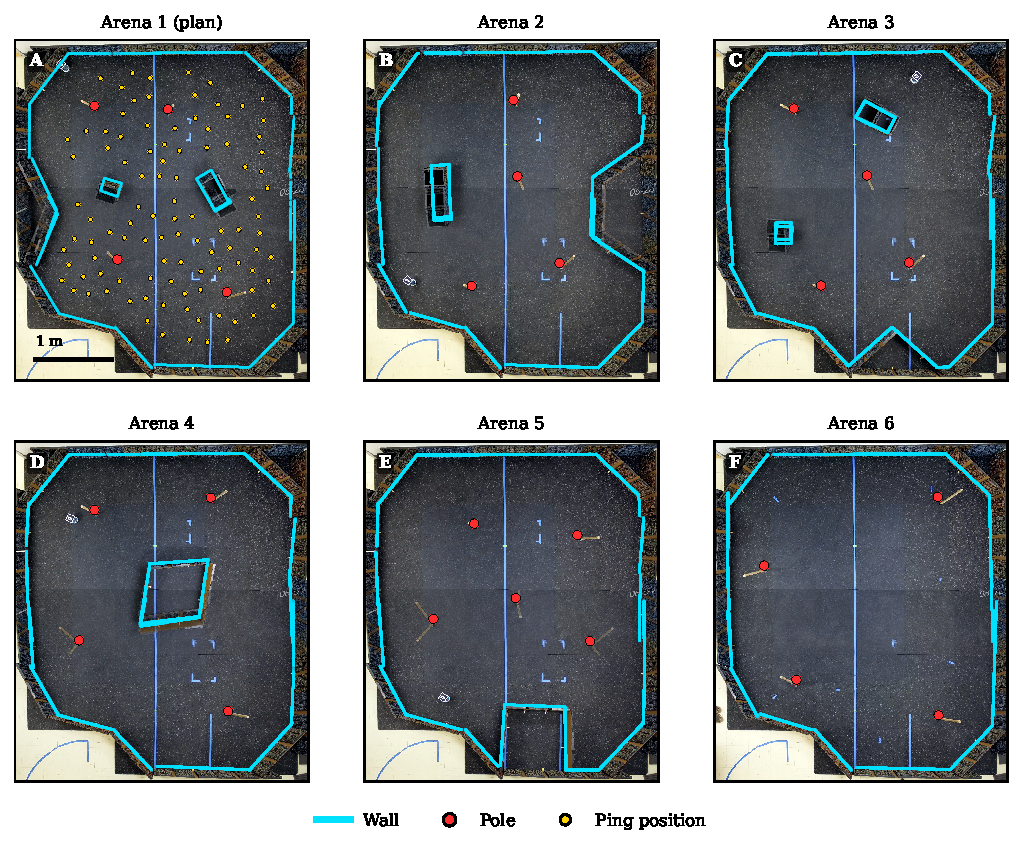
\includegraphics[width=0.85\textwidth]{fig_arena_layouts}
	\caption{Arena layouts for collecting inverse-model training data. We recorded echoes in six arenas, each sharing an overall outline set by the overhead camera's field of view. Within that outline, we moved boundary walls, installed interior walls, and placed four or five poles at semi-random positions, so that the sessions sampled a range of geometries. All panels are overhead images with the digitized geometry overlaid (walls, cyan; poles, red; ping positions, yellow). Panel A shows arena 1 together with the positions at which the robot ensonified it, the sampling scheme used in every session; panels B to F show arenas 2 to 6 with their geometry alone. Arena 6 (F) differed from the others in both its layout and its sampling headings (see text). All panels share the scale bar (1\,m) shown in panel A.}
	\label{fig:arena_layouts}
\end{figure}

For each session, we used a predetermined number of semi-random positions within the arena (see Fig.\ref{fig:arena_layouts}A for an example). We sequentially drove the robot to each position using the overhead camera system. Once the robot arrived at a position, it rotated to five headings, emitted one sonar pulse at each, and recorded the resulting echo envelopes at both ears. In the first five sessions, these five headings were spaced $72^{\circ}$ apart. The emitter, modeled as a 15\,mm-diameter circular piston at 42\,kHz, has a $-6$\,dB main lobe about $\pm 22^{\circ}$ wide; at $\pm 35^{\circ}$ off axis, its directivity falls by roughly 18\,dB. Because successive headings were $72^{\circ}$ apart, well beyond this main lobe, the five emissions sampled approximately non-overlapping, and therefore approximately independent, regions of the environment.

The first five arenas could not supply echoes from distant reflectors. Their interior walls and their outlines limited the closest reflector to about $2.1$\,m. This left the inverse model untrained over much of the range at which the sonar still returns usable echoes. We laid out the sixth arena to address this. We left the interior unobstructed and placed only four poles well clear of the walls. In this arena, the in-cone range of the closest reflector extended to $3.2$\,m. In this session we also chose the headings based on the arena's geometry rather than uniformly: at each position, three of the five pointed down the longest available sight lines and the other two filled in, subject to a minimum separation of $40^{\circ}$. That separation is narrower than the $72^{\circ}$ used elsewhere, so adjacent emissions in this session could overlap slightly at the edge of the main lobe, and the independence argument above applies to the first five sessions only. The session yielded $314$ echoes whose nearest reflector lay between $1.5$ and $3.5$\,m, against $11$ beyond $1.7$\,m in the five earlier sessions combined.

Across the six sessions, we collected 2775 binaural echoes through systematic sampling. For perspective, \animal{ef} emit calls at 10--20 per second \citep{Barchi2013}, so 2775 echoes represent under 5 minutes of call data. Even accounting for our efficient sampling, a bat could likely gather comparable data over typical experimental timeframes. For example, \citet{Barchi2013} flew bats for at least 5 minutes per day over 6 successive days. In the field, each night, bats seem to emit 1000s of calls per night. \textit{Myotis} species commute at up to 7 m/s while emitting more than 10 calls per second \citep{Holderied2006,Schaub2007}, so 2775 calls correspond to under $2$\,km of flight. \citet{Arlettaz1999a} recorded mean one-way distances between the nursery roost and the foraging grounds of $8.7$ and $3.9$\,km in \animal{mt} and \animal{mb} respectively, with the farthest feeding grounds at $25$\,km.

For each robot position and orientation, we also collected a visual snapshot using the overhead camera system to record the local geometry. We modeled our robotic bat with a visual field of $\pm35^{\circ}$ for two reasons. First, this coincides with the approximate width from which the robot received echoes from the walls and poles, thus matching the sonar system's field. Second, a field of this width is biologically plausible for a bat, lying between the binocular ($50^{\circ}$) and monocular ($120^{\circ}$) visual fields measured in the gleaning bat \animal{mc} \citep{Bell1986}. Within this field, we extracted the nearest reflector from manual annotations marking walls and pole locations on the overhead arena view. This nearest reflector set the ping's class label: \emph{wall} or \emph{pole}. We placed no upper limit on the labeled range, so a reflector several meters away was labeled by its true class rather than treated as absent: $930$ of the $2775$ echoes had their nearest reflector beyond $1$\,m, the most distant at $3.2$\,m. The label set also includes a third value, \emph{none}, for a cone holding no reflector at all, but none of these six sessions included it. The robot always recorded from inside a closed arena, so some part of a wall fell within the $\pm 35^{\circ}$ cone at every pose it occupied. 
%
The third output of the classifier therefore received no training examples, and the deployed model is in practice a two-way classifier: over all $2775$ echoes, the largest probability it assigns to \emph{none} is $6.5\times10^{-4}$.
%
For a pole, we recorded azimuth (relative to the robot's heading, as a signed angle) and range (to the pole's surface rather than its center). For a wall, we recorded a coarse three-direction depth profile: we divided the $\pm 35^{\circ}$ cone into left, center, and right thirds, each about $23^{\circ}$ wide, and set each direction's depth to the nearest wall distance within its third, resulting in a very coarse depth profile.

\subsubsection{Inverse-model architecture and training}
\label{sec:inverse-training}

We implemented the inverse model as a convolutional network (Fig.~\ref{fig:network}). A shared trunk of one-dimensional convolutions, pooling, and a fully connected layer encodes each ear's envelope into a 32-element embedding ($z_L$ and $z_R$). Five output heads use these embeddings: \emph{classification} (wall or pole), \emph{depth} (the three wall distances), \emph{azimuth} (the pole's azimuth), \emph{pole range} (the pole's distance), and \emph{nearest-reflector range} (the distance to the nearest reflector, whatever its class). The last four are heteroscedastic regression heads, each returning both a value and a variance, giving every distance and bearing an uncertainty estimate.

To a first approximation, the two ears are symmetric. Swapping the echoes should therefore yield the same class, a depth profile with left and right exchanged, an unchanged pole range, and a pole azimuth of opposite sign. We enforced symmetry by combining the embeddings into two 64-element vectors:
%
\begin{equation}
	z_{LR} = [\,z_L,\, z_R\,], \qquad z_{RL} = [\,z_R,\, z_L\,],
\end{equation}
%
We run each of the five heads twice, once using $z_{LR}$ as input and once using $z_{RL}$ as input. We then average the outputs after flipping the depth-head output and the azimuth-head sign for $z_{RL}$. The class and range heads needed no correction, as their outputs are unchanged by the swap, so we averaged them directly. We combine the predicted variances symmetrically, as we do for the depth means. Encoding symmetry this way forces the model to respect it exactly. It also roughly doubles the effective training data (each emission serves as its mirror image) and reduces the parameter count. This symmetry constraint is not strictly necessary: a variant without it, free to learn left-right asymmetries, fit the depth profile slightly worse (data not shown). Table~\ref{tab:inverse-params} lists the configuration.

\begin{figure}[htb]
	\centering
	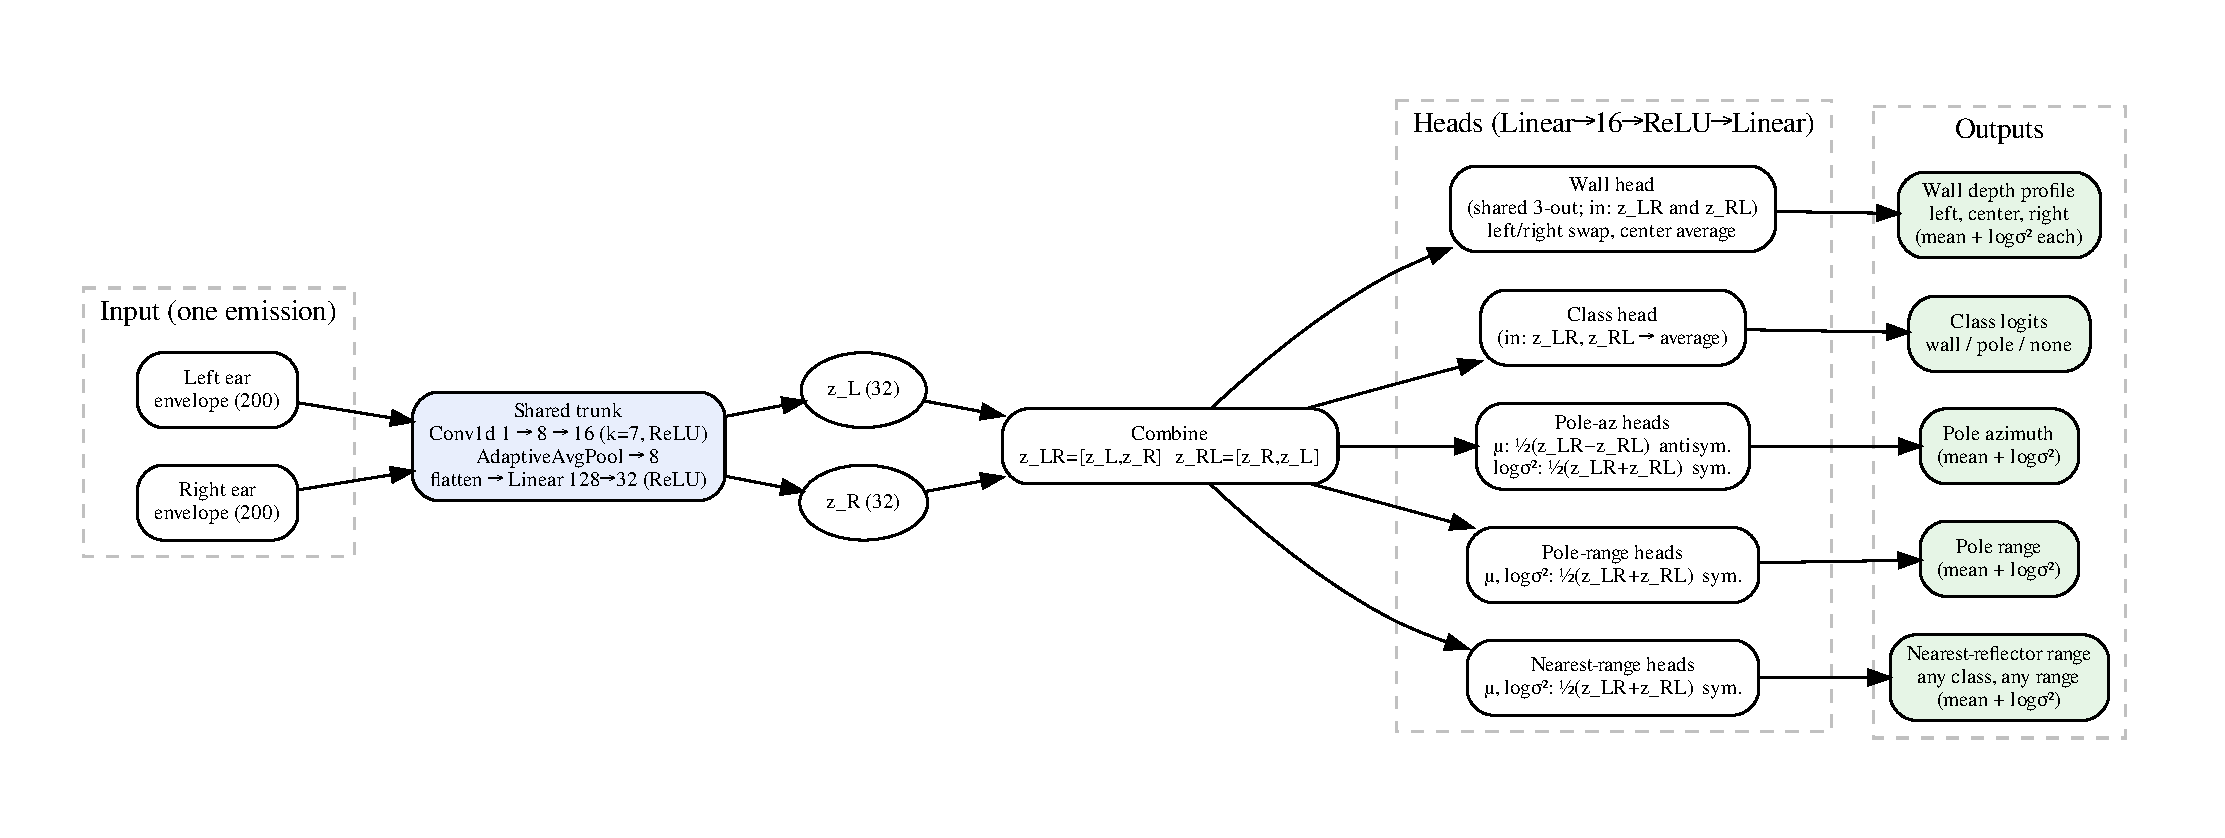
\includegraphics[width=\textwidth]{fig_network}
	\caption{Architecture of the convolutional neural network we used to implement and train the inverse model. An emission produces one echo envelope per ear (200 samples), which a shared trunk encodes into 32-dimensional embeddings $z_L$ and $z_R$; these feed five output heads: classification, wall depth, pole azimuth, pole range, and nearest-reflector range. \emph{Combine} forms the two ear orderings $z_{LR}=[z_L,z_R]$ and $z_{RL}=[z_R,z_L]$. Each head consists of a small two-layer network. The \emph{wall} head is a single three-output head applied to both orderings, giving the nearest-wall distance in the left, center, and right thirds of the field of view; the swap exchanges its left and right outputs, so those two distances are read from the two orderings, while its center output is averaged over them. The \emph{class} head averages its output over both orderings, giving a wall/pole prediction that is unchanged when the ears are swapped, and the two \emph{range} heads are averaged in the same way, since a reflector and its mirror image lie at the same distance. The \emph{pole-range} head is trained only on echoes whose nearest reflector is a pole within $1$\,m, and supplies the terminal approach stop; the \emph{nearest-reflector-range} head is trained on every echo at every range, and so answers a question that needs no classification. The \emph{pole-azimuth} mean is the only antisymmetric output, $\tfrac{1}{2}(z_{LR}-z_{RL})$, and so flips sign with the swap. The four regression heads are heteroscedastic: each returns a mean and a log-variance, $\log\sigma^2$, the latter expressing the model's per-estimate uncertainty.}
	\label{fig:network}
\end{figure}


We trained the model by minimizing a five-part objective, each part carrying equal weight: a cross-entropy classification loss and four regression losses, for the wall depth profile, the pole's azimuth, the pole's range, and the nearest reflector's range. The classification loss used all echoes for each emission. We applied three of the regression losses as \emph{masked} losses, considering only the relevant classes, so the depth profile was fitted on wall echoes and the azimuth and pole range on pole echoes. We further restricted the pole-range loss to poles within $1$\,m. That head supplies the terminal approach stop, and widening the span it is trained on degrades it at close range, where the stop decision is taken. The nearest-reflector range loss carried no mask: we applied it to every echo at every range, which is what lets that head report a distance for a reflector it cannot name. All four regression losses were Gaussian negative log-likelihoods: each weights the prediction error by the model's predicted variance and penalizes it, so the network learns to report a calibrated per-estimate uncertainty rather than a point value alone.

We optimized with Adam (learning rate $10^{-3}$, batch size 64) for 60 epochs. For the first 20 epochs, we trained the regression means with a plain squared-error loss before enabling the variance terms, which stabilized early training. We rescaled four quantities for training: standardized input envelopes, pole-azimuth targets divided by the cone half-angle, and both range targets divided by $1000$\,mm, placing all regression targets on a common scale. For the nearest-reflector range, that divisor is a scale rather than a limit: the head was trained on targets beyond it and predicts beyond it.

We trained five different versions of the inverse model on the data from all six sessions. We used the first four versions as benchmarks, while the fifth version was the deployed model. To train the first four variants, we divided each session's recording positions into four spatial quadrants and held out one quadrant in turn (roughly a quarter of the echoes), training four models. We refer to these models as quadrant models in the remainder of the paper. Because the quadrants partition the data, each echo was held out exactly once, and we evaluated it with the model that was not trained on it. This gives a held-out estimate across all $2775$ echoes, which matters for results that vary with range, where a single held-out patch leaves too few echoes in each range band.

To train the fifth, deployed, model, we held out $15\%$ of the echoes as a single contiguous patch for each session, those collected nearest a randomly chosen location, trained on the remaining $85\%$, and used the patch for early stopping. Because a patch is a coherent region of the arena rather than a scatter of poses, it consists of locations the model never trained on. Hence, the gap between training and held-out performance is an overfitting check (Table~\ref{tab:inverse-results}), in addition to the comparison with the first four models.

In the results, we compare the performance of the  four quadrant models with that of the deployed model. This comparison allowed us to assess whether the performance we obtained for the deployed model is stable or depends on idiosyncratic (spatially coherent) samples in the dataset. If the deployed model's performance matches that of the quadrant models, we can assume it is stable and does not depend on specific training samples. Beyond this, we did not use a separate validation set, and we consider successful task completion validation of the deployed model. 

\subsection{Experiment 1: obstacle avoidance and target approach}

In Experiment 1, we asked whether the noisy inverse model could drive simple navigational behavior from sonar alone. The arena had a single pole. The robot had to approach the pole while avoiding walls, using features provided by the inverse model: the nearest reflector's class, and either the pole's azimuth and range (when a pole is nearest) or a coarse wall-distance profile (otherwise). This task is analogous to prey-capture experiments where bats approach objects at unknown positions, e.g., tethered insects \citep{Ghose2003}, mealworms \citep{Falk2014}, or artificial flowers \citep{Simon2011}.

As a comparison, in addition to the sonar-only runs, we also ran vision-only experiments using the overhead camera system. At each step, regardless of the modality used, the robot received a single local feature description of the nearest reflector within its forward $\pm 35^{\circ}$ field. This description included the reflector's class and matching geometry: pole azimuth and range for poles, and a three-direction depth profile for walls. For sonar, we used the inverse model's output for the binaural emission acquired at the robot's current pose. For vision, we used the overhead camera's digitized arena geometry at the robot's current pose, taking the nearest reflector in the same $\pm 35^{\circ}$ cone. Crucially, we supplied only this local feature from the robot's instantaneous pose, never a map of the arena. Although the overhead camera held the complete arena geometry, we restricted the controller to querying it only within the same forward cone as the sonar inverse. Thus, the overhead camera system modeled a bat's local visual field.

Our vision model implied that perception was stroboscopic for vision as well as for sonar: the robot perceived the environment once per step. Although bat sonar is inherently stroboscopic, vision is not. Nevertheless, we modeled vision as intermittent to match the sampling rate of the two conditions. The modalities were not matched in range, however. We did not range-limit vision, whereas the sonar inverse model grows unreliable with distance. This range asymmetry reflects the difference in operational range between sonar and vision \citep{Boonman2013}. The inverse model was trained on echoes up to $3.2$\,m, but its discrimination of the nearest reflector's class degraded beyond roughly $1.4$\,m. We therefore ignored poles reported by the model whenever the class-agnostic range head placed the nearest reflector beyond $1200$\,mm. This prevented the robot from acting on an identification made at a distance where walls and poles are no longer separable. %The wall channels carried no such veto, since the depth profile steers away from a surface rather than identifying one.

We hand-coded the mapping from local features to motor commands rather than learning it. Bats could acquire such mappings through learning over repeated trials \citep[e.g.,][]{Ghose2003,Falk2014,Simon2011,Holland2005,Finger2025}. We did not model this learning because the question we consider in this paper is not how bats learn to use the inverse but whether the cross-modally trained inverse delivers sufficiently reliable features for such learning to be possible. The fixed rule therefore stands for the association a bat would acquire through reinforcement. It holds no map of the arena, and beyond two counters, of consecutive steps with a wall close by and of consecutive pole detections, it keeps no memory of earlier observations. Nothing accumulates that could compensate for a poor estimate, so the behavior reflects what the inverse model delivers step by step.

The robot used the extracted feature as follows. When perceiving no pole and either no wall or a wall further than 750\,mm away, it wandered through the arena in a slight curve, covering 150\,mm between measurements. We re-randomized the curvature on each wall contact so that repeated encounters did not send the robot along the same arc. In lab experiments, the bat \animal{ef} flies at about 2.5 m/s while emitting 10 to 20 calls per second \citep[e.g.,][]{Barchi2013}, covering roughly 125 to 250 mm between successive calls. The robot's 150 mm step falls within this range. Hence, while we did not aim to model a specific species, this indicates that the distance traveled between acquisitions is biologically plausible.

When the robot perceived a wall nearby, it took evasive action. A wall within $750$\,mm triggered a reflection, causing the robot to turn away by an angle derived from the three slice depths, and it drove on only while the wall was not immediately ahead. A wall persistently close in all three directions (as would be caused by a corner) triggered a large escape turn toward the more open side. When perceiving a \emph{pole}, the robot turned toward the feature's azimuth by a fixed fraction of the bearing (capped at $25^{\circ}$ per step) and advanced a fixed step. Applied repeatedly, this curves the path onto the pole. We reduced the displacement between sensory acquisitions to $75$\,mm to model the increased call rate and reduced flight speed of bats approaching a target. In \animal{ef}, the rate rises from 2 to 10 calls per second while searching to as much as 200 per second in the terminal buzz \citep{Ghose2006}. Either an increase in rate or a decrease in speed shortens the distance flown between calls, and halving the step models that shortening: at the cruising speed above, $75$\,mm corresponds to about 30 calls per second, between the search and buzz rates reported for this species. Practically, the smaller steps during the pole approach also resulted in the robot reporting pole detection for more steps, enabling us to assess the stability of the detection. Table~\ref{tab:controller-params} lists every constant of the controller together with what it governs.

We selected five different start poses for the robot in the arena. For each, we tested the robot to find the pole at two positions using sonar or vision. Hence, we ran 20 runs (5 start poses $\times$ 2 pole positions $\times$ 2 modalities). Each run began from its start pose and proceeded in discrete sense-act steps until one of four outcomes: the robot arrived at the pole, collided with a wall, became trapped in a corner, or reached a limit of $200$ steps. We judged arrival on the robot's own perception. We marked the robot as having arrived at the pole if the perceived pole range was less than $400$\,mm and the pole was perceived on three consecutive sensory acquisitions. Once the robot arrived at the pole, it regulated the perceived bearing toward zero by turning in place by a fixed fraction of the perceived bearing, re-sensing after each correction, and giving up after ten iterations. We required the robot to null the azimuth to demonstrate that it perceived not only the pole's distance but also its azimuth. We set the stop criterion at $400$\,mm rather than at contact because the inverse model has no training data closer than $249$\,mm; the acquisition planner held every waypoint $250$\,mm clear of all reflectors, so any range estimate below that distance is an extrapolation, in exactly the regime the stop decision would occupy. In addition, the emission occupies roughly the first $1.5$ to $2$\,ms of each recording, so an echo returning from closer than about $300$\,mm arrives while the sensors are still emitting. A stop at $400$\,mm places the final range estimate just outside this overlap. Earlier work with these same sensors used a comparable criterion \citep{Vanderelst2026}.

\subsection{Experiment 2}

In the second experiment, we asked whether the inverse model can support a more complex task. We selected a task inspired by the stable flight paths observed in bats, both in experiments \citep{Barchi2013} and in the field \citep{Holderied2006}. In particular, we modeled a bat that has learned to fly a stable route and, while flying it, with both vision and sonar available, learns to associate the features its sonar recovers at each point with the motor commands that keep it on the route, i.e., those features for which it has an inverse model. Once the bat learns the association, it could fly the same route supported by sonar alone. Currently, it is unknown whether bats can transfer route following learned through vision (alone) to sonar. Although this could be tested under experimental conditions, bats in the wild would always have access to sonar. However, for this paper, i.e., demonstrating that a noisy inverse model supports non-trivial behavior, this scenario is a good test case.

To determine the path the robot should follow, we drew a closed loop over the digitized arena, along with a rectangular release box and a release heading, and resampled it at $25$\,mm spacing so any position could be expressed as a distance traveled along the loop. We implemented the controller as a recurrent network with $32$ hidden units. At each step, it received the same local feature the inverse model supplies in Experiment 1, together with the rotation it commanded in the previous step, and returned a rotation, capped at $90^{\circ}$, after which the robot drove forward $150$\,mm. Because the network is recurrent, it can combine what it senses now with what it sensed earlier. The rotation fed back is the one the network commanded, not the one the motors executed: the robot has no odometry, no inertial sensor and no access to its own position. Since those commanded rotations were themselves computed from earlier echoes, the network's state at any step is a function of the echoes it has heard and of nothing else. Any record it keeps of where it is on the route is therefore built from sonar.

We trained the controller in simulation to associate the arena's local features with the motor commands that keep the robot on the path. We did not model how the route was chosen, or where the corrections that keep the robot on it (while using vision) originate. In other words, we assumed that the bat already knew how to follow the path visually. We only modeled acquiring a controller that could mimic the path using sonar, using the features extractable by the inverse model. A pure-pursuit controller with access to the robot's true position drove the route, projecting that position onto the loop, advancing $240$\,mm along it, and returning the rotation that pointed at the resulting target. We trained the controller with no access to the robot's position. It received only the local feature and the rotation it had commanded on the previous step, so that it could learn only those associations that features recoverable from sonar can support. The features presented during training carried realistic error, drawn from the errors the inverse model makes on real echoes.

We applied two kinds of perturbation during training. First, on $30\%$ of steps we disturbed the commanded rotation by about $30^{\circ}$ while keeping the clean rotation as the training target, so that the controller also learned to return to the path after leaving it. Second, the simulated motors did not execute commands exactly. Besides a small per-step error, we gave each episode two sustained faults of the kind the real robot shows, each drawn once at the start of an episode and held for its whole duration: a gain error of up to $15\%$ in rotation and $5\%$ in distance, and an additive rotation bias of up to $5^{\circ}$, applied at every step. The additive term models drive curl, the robot's dominant fault: it turns slightly while driving forward by an amount unrelated to the commanded rotation, so a multiplicative gain error cannot reproduce it. Neither fault averages out over a lap. Hence, the controller could not hold the path by counting its own movements alone and had to learn to compensate for long-term drift in its position from what it sensed.

We then deployed the trained controller on the robot, released it from the release box, and let it run for several laps. We first ran the arena as we had trained the controller, and repeated that run. The difference between these two runs sets a standard against which the effect of any manipulation can be judged. To test whether the robot actually used what it sensed, we then ran conditions in which we removed or displaced objects (see the results section for details of the manipulations). The alternative is not path integration in the usual sense, since the controller has no self-motion signal to integrate, but that its recurrent state runs as a nearly autonomous pattern, replaying the route while barely consulting the current echo. If what the robot senses does not matter, the route should be unchanged. If it uses what it senses to stay on track, the route should change. We manipulated the arena rather than the sensory input itself because the controller's input has no null value: every feature the inverse model reports is a claim about the world, so sensory data cannot be withheld, only replaced with a false reading. We repeated the procedure in a second arena, with its own path and controller.

For every run, we logged the robot's trajectory from the overhead camera system. We report the number of laps completed, the distance from the path at each step, and, in the conditions where we displaced an object, how far the trajectory shifted toward its new position. 

\dnote[18]{\emph{Interpretation item, not a Methods gap.} Nothing in this subsection needs changing; what is missing is how to \emph{read} the manipulations, and that belongs in the Experiment 2 Results and the Discussion. Three things the data already constrains. (1) The non-separability argument above justifies the design but limits the reading: a null result under a manipulation cannot by itself mean the robot ignored that object, since the contribution could be present and swamped. (2) What rescues it is a dissociation. Removing the poles moved the route, while displacing them twice, in different directions, did not. For thin dowels presence matters and position barely does, and neither result alone would support that. (3) The walls behave oppositely: a displaced wall captured the route almost completely, so there position is nearly everything. Together these say the controller navigates on boundary geometry and object presence rather than object identity. That is the sense in which \emph{landmark} can be used here, and it is what makes the Neuweiler and M\"ohres (1967) \emph{Raumbild} the right precedent (scratchpad section 6).}

\section{Results}

\subsection{Inverse model}

We trained 5 different versions of the inverse model: four quadrant models and the deployed model (Section~\ref{sec:inverse-training}). Fig.~\ref{fig:perception-examples} shows what a single perception looks like, and may be worth consulting before the aggregate results below. Each of the $2775$ echoes was interpreted by whichever quadrant model had not been trained on it. On average and across distance to the nearest reflector, the quadrant models recovered the class of the nearest reflector on $79.4\%$ of echoes. The deployed model correctly classified $79.2\%$ of $418$ echoes, making the performance similar. Fig.~\ref{fig:inverse-results} compares the classification performance of the four quadrant models and the deployed model as a function of distance. This figure also shows the majority class, i.e., the percentage of walls or poles, whichever is the most prevalent in the respective distance range. This percentage serves as the baseline for the model’s performance. This shows that beyond about $1500$\,mm, the models perform worse than baseline and can no longer correctly classify the closest object (in the visual field, which provided the ground truth) as a pole or a wall.

The classifier emits a probability for each class. Fig.~\ref{fig:inverse-results}A reports how often the most likely one was correct. Fig.~\ref{fig:inverse-results}B plots how often the model was correct as a function of the probability the model reported. Points on the diagonal mean the reported probability can be taken as a probability of the class membership. The model stays close to the diagonal: when it reports being $90\%$ certain, it is correct on $97.8\%$ of those echoes. This is useful for a controller, which can act on the class where the model is confident and disregard it where it is not, without the model needing a separate category for \emph{unsure}.

\begin{figure}[!htbp]
	\centering
	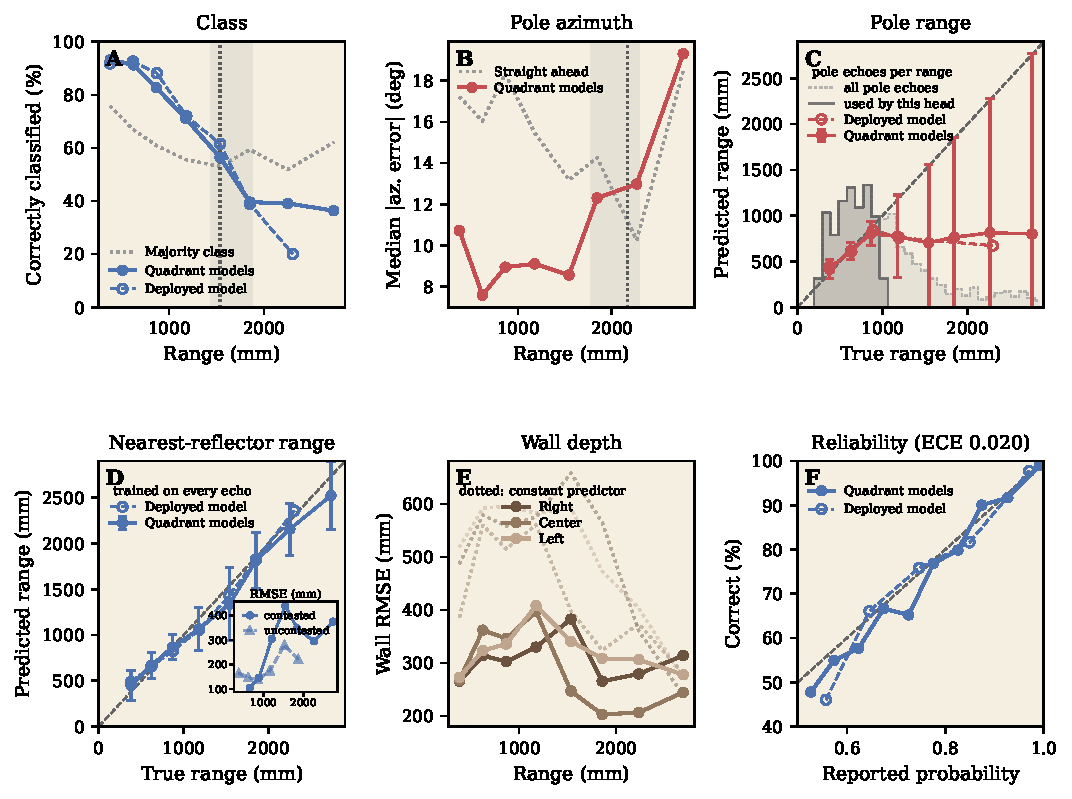
\includegraphics[width=0.92\textwidth]{fig_inverse_limits}
	\caption{What the inverse model recovers, as a function of the range to the nearest reflector in the analysed $\pm 35^{\circ}$ cone. Solid lines with filled markers are the four quadrant models, every one of the $2775$ echoes scored by the model that did not train on it. Dashed lines with open markers are the deployed model on its own held-out $15\%$, drawn only in bands holding at least $15$ of those echoes, which is why they stop short of the longest ranges. Grey dotted lines are baselines rather than models.
(A) Classification accuracy, against the majority class of each band: the score obtainable by ignoring the echo entirely. The vertical dotted line marks where the models stop beating that baseline, $1537$\,mm, and the shaded band is its $95\%$ bootstrap interval.
(B) Reliability of the class posterior: the probability the model reported against how often the class it reported was correct. The deployed model is binned into five probability intervals against the quadrant models' ten, since it is scored on $418$ echoes rather than all of them.
(C) Median absolute error in pole azimuth, against the error of always answering straight ahead, which the models stop beating at $2168$\,mm. The deployed model is not drawn here: it could be scored on only $17$ to $23$ pole echoes per band, whose bearings are easier than those the baseline is computed over, so the two are not comparable.
(D) The pole-range head, which is trained only on poles within $1$\,m. The histograms give pole echoes per range, all of them as a dashed outline and the subset this head was trained on filled; their heights are scaled for visibility, so only the relative counts and the edge at $1$\,m carry meaning. Bars are the standard deviation of the predictions rather than the error: beyond its training span the head does not become uncertain, it becomes constant.
(E) The class-agnostic range head, trained on every echo at every range, drawn on the same axes as (D) for comparison; bars are $\pm$RMSE. The inset gives RMSE against range separately for echoes with and without a nearer reflector just outside the cone, and stops at $2$\,m because uncontested echoes become too rare past it.
(F) Wall-depth error for the three directions, against a constant predictor that answers each band's mean distance and never listens (dotted, in the matching colour).}
	\label{fig:inverse-results}
\end{figure}


Fig.~\ref{fig:inverse-results}C shows the error of the models in predicting a pole’s azimuth from the echoes, again as a function of distance. We compare the models’ performance with a baseline for a model that returns 0 degrees, irrespective of the input. This plot shows that the quadrant models stop outperforming the baseline at around $2000$\,mm. The deployed model still seemed to outperform the baseline beyond this distance (not shown). However, this compares the deployed model against a baseline computed over all echoes, rather than over the small sample of $23$ echoes beyond $2000$\,mm on which the deployed model could be scored. Measured on those same  $23$ echoes, the baseline error is $4.9$ degrees, and the deployed model achieves $6.8$. Hence, just like the quadrant models, the deployed model does not outperform the baseline beyond $2000$\,mm either. 

Fig.~\ref{fig:inverse-results}D shows the performance of the models for pole range. This plot shows that, even though the model can recognize a pole as such up to $1500$\,mm (Fig.~\ref{fig:inverse-results}A), the estimated distance saturates at about $800$\,mm. Poles farther than about $800$\,mm are perceived as closer than they are. This is due to a training decision we made. We trained the pole-distance head only on echoes where the pole was the closest object and less than $1$\,m away (See histograms in Fig.~\ref{fig:inverse-results}D). We did this because training the model on all available echoes where the pole was the closest introduced bias and increased distance-prediction error at short range {Fig \ref{fig:pole-range-cap}}.  Given this trade-off, we trained the model to improve pole-range inference at short ranges, at the cost of not being able to localize poles beyond about $1$\,m. However, this job was partially fulfilled by the class-agnostic distance prediction, which we discuss in the next paragraph. Fig.~\ref{fig:pole-examples} shows the consequence echo by echo. Within a metre the model's estimate falls on the pole; beyond it the estimate stops moving outward as the pole recedes, and the classifier's confidence that it is looking at a pole at all falls away with it.

\begin{figure}[!htbp]
    \centering
    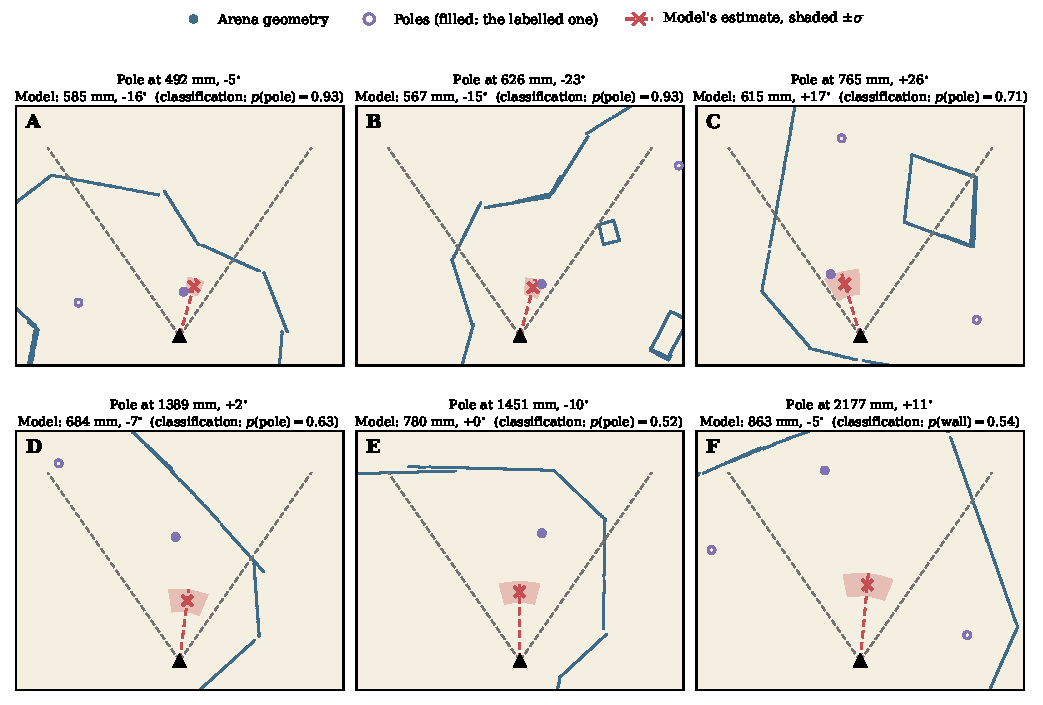
\includegraphics[width=\textwidth]{fig_pole_examples}
    \caption{What the model reports about a pole, for six individual echoes, one per range band. The layout follows Fig.~\ref{fig:perception-examples}: the robot sits at the apex with its field of view pointing up, and blue marks the digitised arena. The pole the echo was labelled with is filled purple; other poles are open circles. The red patch is the model's estimate, the predicted bearing with its $\pm\sigma$ as an angular wedge crossed with the predicted range and its $\pm\sigma$ as a radial band, and the cross marks the estimate itself. Titles give the true range and bearing, then the reported ones, then the probability the model assigned to the class it reported. Examples were chosen by rule: among the echoes the model classified as a pole, which are the only ones whose pole channels the robot uses, the one whose combined bearing-and-range error is the median for its band. Within a metre (A--C) the estimate falls on the pole, with the range recovered to within a few tens of millimetres. Beyond it (D--F) the range estimate stops moving outward while the pole recedes, so the model reports a pole at roughly $800$\,mm whether the pole is at $1.3$ or $2.4$\,m. In each of these the model does call a pole, so these are estimates the robot would act on. That is the reason the controller of Experiment 1 additionally refuses a pole call when the class-agnostic range head places the nearest reflector beyond $1200$\,mm.}
    \label{fig:pole-examples}
\end{figure}

Fig.~\ref{fig:inverse-results}E shows the performance of the head that inferred the distance to the nearest obstacle (within the visual field of the robot). Inferring the distance to the nearest object may seem straightforward, and this head did work well. However, performance had limits. Fig.~\ref{fig:inverse-results}E shows that as distance increases, the errors increase as well. This is most likely because we ask the model to return the distance to the nearest object inside the visual field. At larger distances, it becomes more likely that objects outside this area return an echo preceding that of the nearest object inside the area. Hence, the model must not only find the closest echo but also reject echoes from objects outside the visual field of view. This interpretation is supported by the inset in Fig.~\ref{fig:inverse-results}E, which splits the echoes by whether an object just outside the visual field was nearer than the nearest object inside it. Errors increased when such an object was present, that is, when the closest reflector could not be seen and introduced an echo that had to be ignored.

Together with the categorization head, this head expands the model’s ability to localize poles beyond the dedicated pole range head. The categorization head may signal that the closest object has some low probability of being a pole, while the category-agnostic distance head could return the approximate distance. 

Fig.~\ref{fig:inverse-results}F shows the performance of the 3-segment wall distance prediction. This shows that the prediction outperformed a baseline across most of the distance range in the training set (we show only the quadrant models’ performance to reduce plot complexity). However, average errors were substantial: about $270$\,mm close in, rising to about $400$\,mm between $1$ and $1.4$\,m before falling again at longer ranges.  Hence, while range is easily extracted from sonar, this plot shows that a more difficult task, i.e., extracting the range to obstacles in different directions (i.e., reconstructing a very rough wall profile), is substantially more difficult. Fig.~\ref{fig:perception-examples} shows what this looks like for single echoes. The error is rarely spread evenly across the field: in most examples one sector is recovered almost exactly while another is out by several hundred millimetres, and which sector fails varies from echo to echo.

\begin{figure}[!htbp]
    \centering
    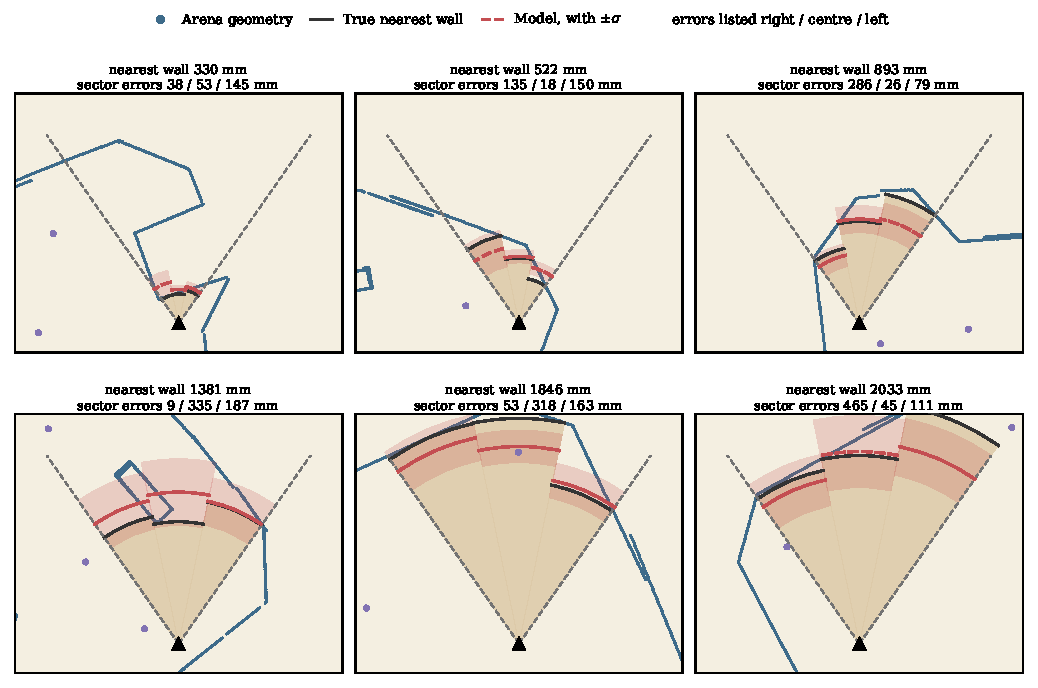
\includegraphics[width=\textwidth]{fig_perception_examples}
    \caption{Six individual perceptions of the wall profile, one for each range band. The robot sits at the apex of each panel with its field of view pointing up; blue marks the digitised arena geometry and purple the poles. In each of the three sectors, the filled wedge reaches the true distance to the nearest wall, the black arc marks that distance, and the dashed red arc is the model's estimate with its predicted $\pm\sigma$ shaded around it. The examples were not chosen by eye: within each range band we took the echo whose mean absolute sector error is the median for that band, so each panel is a typical case for its distance rather than a favourable one. All six share one scale, so the widening of the sectors with range is comparable across panels. Titles give the distance to the nearest wall anywhere in the field, and then the three sector errors, listed right, centre and left.}
    \label{fig:perception-examples}
\end{figure}




In summary, we trained an inverse model using visual input from the overhead camera system to convert binaural sonar data into an estimate of the closest object's position (if a pole) and layout (if a wall). Overall, the model was successful, with some clear limits.  (1) For echoes whose nearest object was a pole, it inferred the azimuth better than baseline up to about $2000$\,mm and distance up to about $1000$\,mm. (2) For echoes whose nearest object was a wall, it inferred the closest distance in three sectors in front of the robot better than baseline, but with considerable noise (see Fig.~\ref{fig:perception-examples} for examples). (3) However, it could classify the nearest object as a pole or wall better than the baseline only up to about $1500$\,mm. (4) The model could estimate the range to the nearest object of any kind out to about $2500$\,mm, with an error of roughly $10$ to $15\%$ of the true range beyond a meter. Note that (1) and (2) are measured on echoes we know came from a pole or a wall, using the camera as ground truth. Beyond about $1500$\,mm the model cannot supply that identification itself, so the bearing in (1) would be of little use to the robot, which would not know it was looking at a pole. The range in (4) requires no identification, which is why it remains usable. Hence, the model could locate an object well beyond the range at which it could identify it, but even ranging was limited.

\subsection{Experiment 1}


All $20$ runs ended with the robot arriving at the pole and facing it under both sonar and vision. Neither modality produced a collision, a corner jam, or a timeout. The closest any run came to a wall was $212$\,mm using sonar and $216$\,mm using vision, above the $20$\,mm clearance at which we scored a collision. When the stop criterion fired, the robot was between $276$ and $372$\,mm from the pole when using sonar, and between $322$ and $390$\,mm using vision, according to the overhead camera system. While approaching the pole, the robot rotated on each step to regulate the perceived azimuth to zero. As a consequence, when arriving at the pole, the perceived azimuth of the pole was already within $15^{\circ}$, so no final azimuth corrections were needed. The overhead camera system confirms that the robot was indeed facing the pole; at the final pose the pole lay a median of $5.1^{\circ}$ off the robot's heading using sonar (at most $11.2^{\circ}$) and $2.2^{\circ}$ using vision (at most $7.4^{\circ}$). These results show that the inverse model, noisy as it is, was sufficient for the robot to complete the task from every start pose and for both pole placements.


While both sonar and vision allowed the robot to find and approach the pole, as expected, the modalities resulted in very different approach behavior (Table~\ref{tab:direct-results} and Fig.~\ref{fig:direct-results}). Using sonar, the robot took a median of $74$ steps ($12$ to $154$) and traveled $10.16$\,m ($0.84$ to $22.09$), compared to $34$ steps ($13$ to $91$) and $2.64$\,m ($0.76$ to $11.60$) using vision. This difference mainly stems from the limited range over which sonar (and the inverse model) can detect the pole. The sonar runs spent a median of $53$ steps before detecting the pole and an additional $10$ approaching. In contrast, the vision runs needed $4$ steps before seeing the pole and used $25$ approaching. Indeed, vision detected the poles from much farther away than sonar. The robot was a median of $798$\,mm away from the pole when sonar first perceived it, compared to $2038$\,mm using vision. Vision locates the pole from most of the arena, while with sonar, the robot must wander until the pole happens to come within $1$\,m—the distance range we trained the inverse model on. Consequently, the sonar feature was empty on $522$ of the $781$ sonar steps and reported a pole on only $97$ of them, whereas the vision feature was never empty across $410$ steps and reported a pole on $234$ (Table~\ref{tab:direct-results}).


Sonar perception during the runs proved more accurate than the held-out evaluation of the inverse model would suggest. We used the overhead system to compare the perception with the ground truth during the 20 runs in Experiment 1. At each step, we compared the class the inverse reported with the class of the nearest reflector under the tracker's geometry, applying the model's $1$\,m horizon to the ground truth so that a correct abstention counts as correct. Note that the same comparison is not meaningful for vision, which reads its feature from the geometry the tracker also uses to score the run and therefore agrees with it by construction. Over the $781$ steps of the ten sonar runs, the perceived feature category proved correct for $95.0\%$ of steps. Recall reached $93.1\%$ for walls, $86.4\%$ for poles, and $97.5\%$ for the abstain class, and pole precision reached $97.9\%$. Only two of the $97$ steps on which the robot reported a pole were mistaken. These figures exceed what the same model achieves on the held-out echoes (Table~\ref{tab:inverse-results}), where accuracy is $80.1\%$, pole recall $63.3\%$, and pole precision $75.0\%$. The model is the same, but we used a simpler arena than those used during acquisition. The Experiment 1 arena held a single pole, whereas we collected the training echoes in arenas holding four or five, so that in $44\%$ of the training echoes a second pole stood in the cone behind the nearest one, a situation that never arose during the runs.  

% I think we don't need to spend time on discussing where the poles were placed. It's probably not directly relevant. Threrefore, this note can be dropped:
%\dnote[17]{RESTORED 2026-08-07 -- this note was written at a33c350 and lost in the language-edit passes without its items being resolved; all three are still open. (1) The 1400-rollout simulation appears nowhere in the paper (the paragraph is commented out at the end of this subsection), so nothing states how the two pole placements were chosen. That belongs in the Methods: the placements were selected by simulating the reactive rule from the recorded starts against a grid of candidate positions, and the same sweep is what establishes the controller ceiling. (2) Methods calls the 20 robot runs \emph{trials} while this subsection calls them \emph{runs}; pick one. (3) RESOLVED 2026-08-21: the P2/S5 sonar run was re-run with \texttt{START=5} and now draws the same controller seed as its vision partner, so all ten pairs are matched.}


%The same comparison cannot be made for vision, which reads its feature from the same digitized geometry the tracker uses to score the run and therefore agrees with it by construction. What the vision runs do measure is the range asymmetry between the two modalities. The vision feature was never empty across $410$ steps, and on $263$ of those steps the nearest reflector lay beyond $1$\,m and was reported regardless. Under sonar the feature was empty on $522$ of $781$ steps, about two thirds of them. Consequently, vision serves as an upper reference, showing what the reactive rule achieves given accurate local perception and an unrestricted horizon, rather than as a control matched to sonar.


%Finally, the reactive rule alone does not account for these results. Given perfect perception, the same controller reached each of $28$ candidate pole positions from every start pose across $1400$ simulated rollouts, without a single collision or corner jam, and every failure it did produce was a timeout. It follows that a collision or a jam on the robot would have been attributable to perception or to drive error rather than to the rule, and neither occurred in either condition. Since the controller holds no memory of earlier observations and no map of the arena, nothing downstream of perception could compensate for a poor estimate. Consequently, the arrivals rest directly on the features the inverse recovered from single sonar emissions.

\begin{table}[ht]
\centering
\caption{Experiment 1 outcomes over the ten start and placement combinations run under each modality. All $20$ runs ended with the robot arriving at the pole and facing it, with no collisions, corner jams, timeouts, or bearing corrections in either condition, so the table reports the measures on which the two conditions differ. Distances and clearances are the overhead tracker's ground truth, not the robot's perception.}
\label{tab:direct-results}
\begin{tabular}{lcc}
\hline
\textbf{Measure} & \textbf{Sonar} ($n=10$) & \textbf{Vision} ($n=10$) \\
\hline
Steps, median (range)                       & $74$ ($12$--$154$) & $34$ ($13$--$91$) \\
Path length, median (range) (m)             & $10.16$ ($0.84$--$22.09$) & $2.64$ ($0.76$--$11.60$) \\
Steps before the pole was first perceived, median & $53$ & $4$ \\
True pole range at first perception, median (mm)  & $798$ & $2038$ \\
True pole distance on arrival, median (range) (mm) & $331$ ($276$--$372$) & $369$ ($322$--$390$) \\
Smallest wall clearance over all runs (mm)  & $212$ & $216$ \\
Steps with an empty feature                 & $522 / 781$ & $0 / 410$ \\
Steps on which a pole was perceived         & $97 / 781$ & $234 / 410$ \\
\hline
\end{tabular}
\end{table}

\begin{figure}[!htbp]
    \centering
    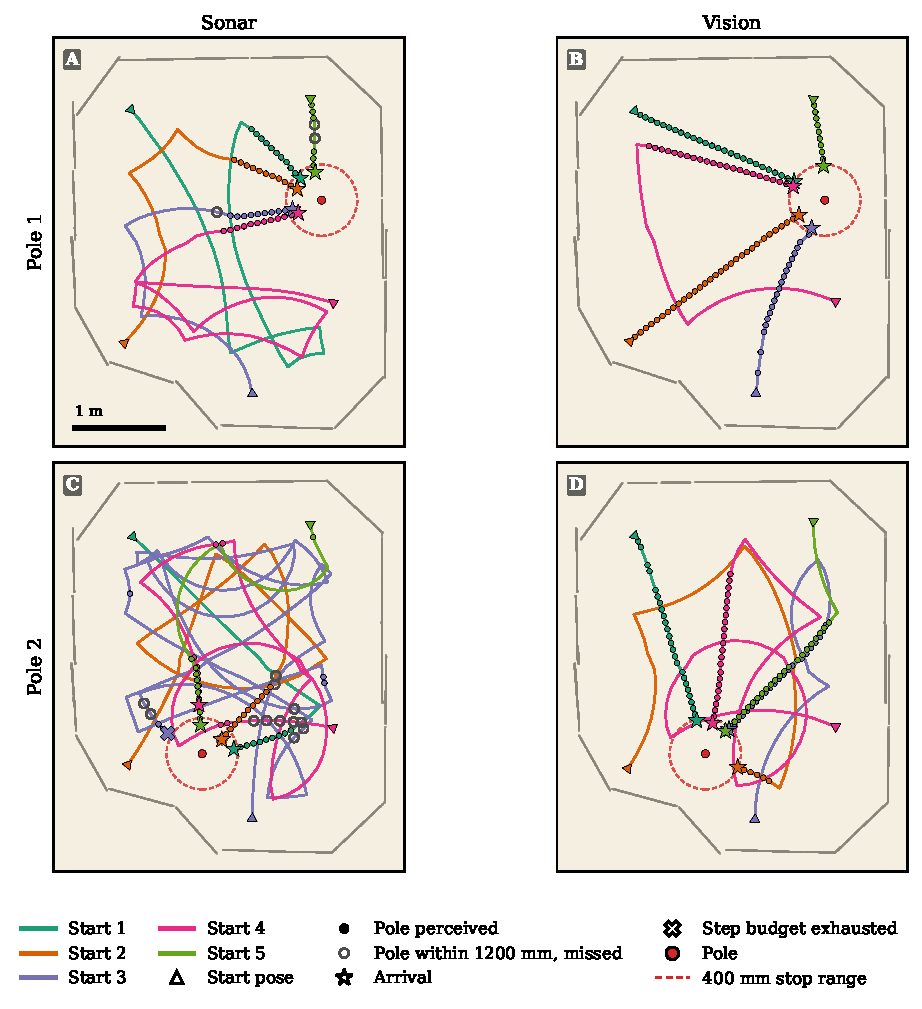
\includegraphics[width=\textwidth]{fig_direct_results}
    \caption{Trajectories of the $20$ Experiment 1 runs. Columns give the modality (sonar, vision) and rows the pole placement. Each panel shows the five runs from the five start poses, one color per start and the same colors in every panel, so that a start can be followed across conditions. Triangles mark the start pose and point along the robot's initial heading, and stars mark the pose at which the run ended. Small filled dots mark every pose at which the modality reported a pole, and open circles every pose at which a pole was the nearest reflector within $1$\,m but went unreported. The pole is the red disc, and the dashed ring is the $400$\,mm perceived range at which the approach stops. Using sonar, the robot wanders until the pole enters the $1$\,m band the inverse model was trained on, so that its detections form a short tail running into the pole (A, C). Using vision, the pole is picked up within a few steps of the start and reported for most of the path (B, D). The missed poles sit at the outer edge of that band, $12$ of the $15$ lying between $800$ and $1000$\,mm from the pole; vision has none, since it reads the geometry the tracker also uses. Two isolated dots in A are the only spurious pole detections of the experiment, at $1373$ and $2233$\,mm from the pole. Note that pole 2 lies close to the arena wall, so that it falls outside the forward cone from several headings even when using vision (D).}
    \label{fig:direct-results}
\end{figure}

\subsection{Experiment 2}

We trained each controller in simulation on the path drawn for its arena (Section~\ref{sec:inverse-training}) before deploying them in the arenas, starting from the release box. Every run lasted for $500$ sense-act steps, allowing the robot to complete several loops of the path. For each path, we completed two runs using the arena layout the controller was trained on. Two runs allowed us to assess baseline variation in the robot's behavior caused by differences in starting position as well as sensory and motor noise. In addition, we completed runs with changes to the arenas, that is, the removal or displacement of poles, blocks, or a wall. The controller was not retrained for these runs.

For every run, we logged the trajectory from the overhead camera system. We report the number of laps the robot completed, its distance from the trained path at each step, and, when the arena changed, the effect of the changes on the robot’s path compared with the variation observed in the two baseline runs. 


\subsubsection{Arena 1}

The first arena held five rectangular blocks and a single pole, and the path was a closed loop of $8.8$\,m. Each run of $500$ steps therefore covered about $8.5$ laps. When run twice without any change to the arena, the robot followed the path closely and repeatably (Fig.~\ref{fig:arena1-runs}A). The median distance from the path was $37$\,mm in both runs, with the ninetieth percentile at $89$ and $94$\,mm and the largest excursion at $188$ and $185$\,mm. Hence, the two runs are not identical, but they show very similar behavior.

Removing the single pole in the arena raised the median distance from the path to $68$\,mm, the ninetieth percentile to $174$\,mm, and the largest excursion to $618$\,mm (Fig.~\ref{fig:arena1-runs}B). We observed increased deviations from the path along the entire loop. However, the deviation was largest around the section of the path nearest to the pole: Fig.~\ref{fig:arena1-runs}E shows a localized peak at about $28\%$ of the loop, where the pole stood ($26\%$). Removing both the pole and one block further increased deviations from the prescribed path to $118$, $370$, and $639$\,mm, and the deviation then peaked at the locations of both removed objects, at about $29\%$ and $68\%$ of the loop (Fig.~\ref{fig:arena1-runs}E).

We displaced two of the blocks by about $320$\,mm and left everything else in place. The route moved with them. Over the stretch of the loop near those blocks, the trajectory shifted $124$\,mm east and $88$\,mm north of the trained path, compared against just $8$ and $9$\,mm in the first baseline run and $19$ and $19$\,mm in the second. That stretch is marked on the path in Fig.~\ref{fig:arena1-runs}D and shaded in Fig.~\ref{fig:arena1-runs}E. The shifts were present on every lap. Away from that stretch, the route was unchanged, so the effect is local to the moving objects. Taking the median eastward offset over that stretch lap by lap gives $156$, $80$, $148$, $111$, $171$, $133$, $158$, $125$ and $105$\,mm across the nine laps, while the same signed measurement on the two baseline runs gives offsets of both signs, with medians of $8$ and $19$\,mm. The deviation as a function of position is elevated over the stretch holding the two moved blocks, which stand at $62\%$ and $70\%$ of the loop (Fig.~\ref{fig:arena1-runs}E).



\begin{figure}[!htbp]
    \centering
    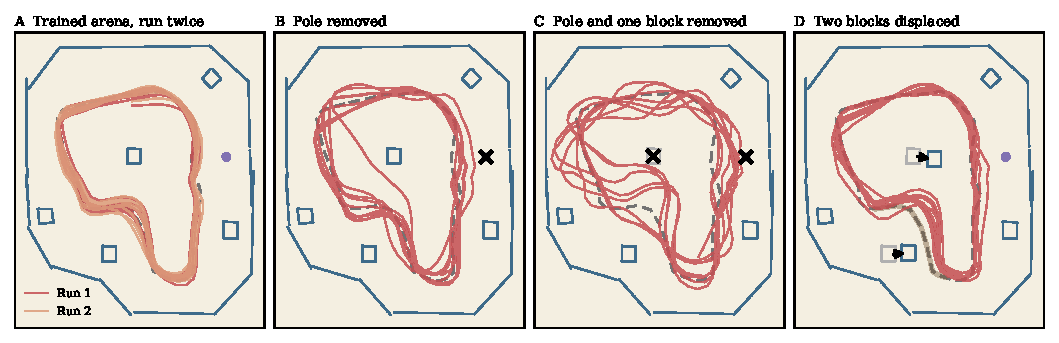
\includegraphics[width=\textwidth]{fig_arena1_runs}
    \caption{Arena 1: the trained route and what each change to the arena did to it. Blue marks the digitised layout, the dashed grey line is the path the controller was trained on, and red is the trajectory the robot flew. (A) The arena as trained, run twice. (B) The pole removed, marked with a cross where it stood. (C) The pole and the central block removed. (D) The central block and the one below it displaced about $320$\,mm east, drawn from their measured new positions with an arrow from where they were trained; the thicker section of the path marks the stretch those blocks border, over which the route shift is measured. (E) The distance from the path against position around the loop, as a median in twenty sections, with the stretch the displaced blocks border shaded. Displacing the blocks lifts that stretch and leaves the rest of the loop at baseline; removing the pole lifts the loop as a whole. The layout drawn in every map is the trained one, which was not re-digitised for the manipulated runs, so removals and displacements are shown from the recorded measurements rather than from a fresh digitisation of each arena.}
    \label{fig:arena1-runs}
\end{figure}


\subsubsection{Arena 2}

Arena 2 had a different outline, five poles and a single block, and the path was a longer closed loop of $11.8$\,m, so each run of $500$ steps covered about six laps (Fig.~\ref{fig:arena2-runs}A). Run twice without any change, the robot again followed the path closely: median distance from the path $43$\,mm in both runs, with the ninetieth percentile at $114$ and $97$\,mm and the largest excursion at $248$ and $183$\,mm.

\begin{figure}[!htbp]
    \centering
    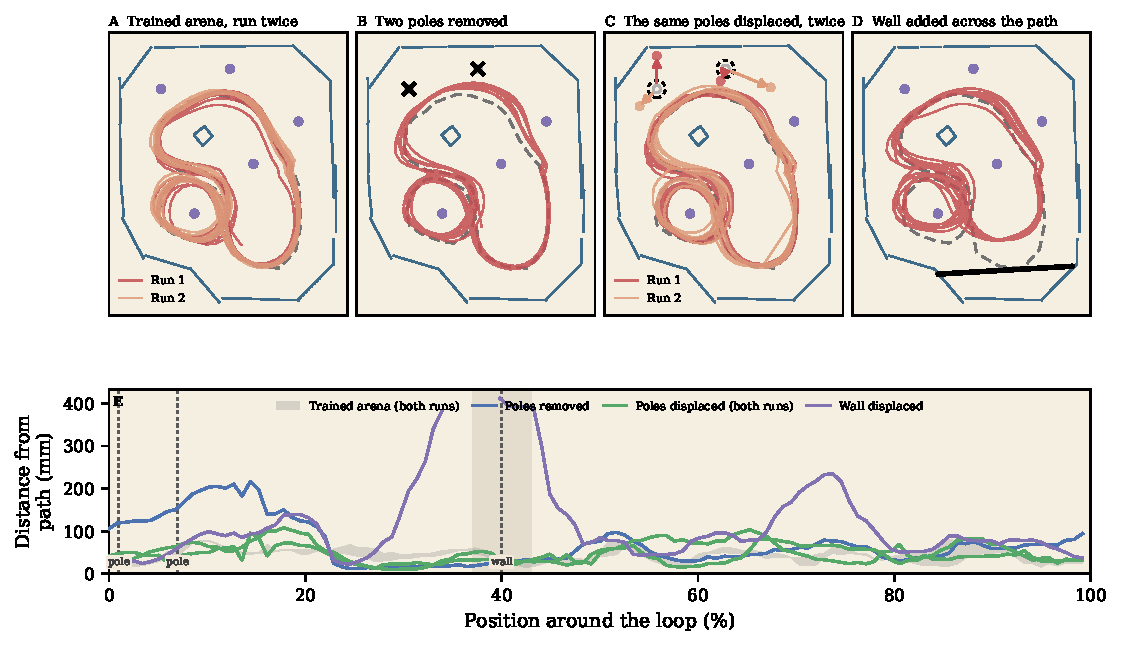
\includegraphics[width=\textwidth]{fig_arena2_runs}
    \caption{Arena 2: the trained route and what each change to the arena did to it, drawn as in Fig.~\ref{fig:arena1-runs}. Blue marks the digitised layout, purple the poles, the dashed grey line the trained path and red the flown trajectory. (A) The arena as trained, run twice. (B) The two northern poles removed, crossed where they stood, and a third displaced (arrow). (C) The same two poles displaced instead of removed, run twice; the first run also carried the third pole at the position it holds in (B). Dashed circles mark their trained positions and the arrows run to where each was measured in that run's own photograph, in the colour of the corresponding trajectory. (D) An extra wall placed across the southern part of the loop, in black, at the position measured from that run's own photograph. The arena's own boundary was left in place, so nothing was displaced here; the new wall stands about $450$\,mm inside the boundary and a few centimetres outside the trained path. (E) Distance from the path against position around the loop, as a median in a sliding window of $500$\,mm of path, with the stretch the added wall crosses shaded and the three manipulated poles and the wall marked. A gap in a curve marks a stretch the robot entered too rarely for a median, which happens where a manipulation pushed the route away from that part of the loop altogether. Removing the poles raises the profile where they stood, displacing them changes nothing anywhere, and the added wall produces a single tall peak where it borders the loop.}
    \label{fig:arena2-runs}
\end{figure}

We removed the two poles standing nearest the northern part of the loop, and displaced a third, standing east of the loop, by about $225$\,mm to the south-west (Fig.~\ref{fig:arena2-runs}B). The median distance from the path rose to $57$\,mm, the ninetieth percentile to $154$\,mm and the largest excursion to $289$\,mm (Fig.~\ref{fig:arena2-runs}B). As in Arena 1, the deviation was concentrated where the removed objects had stood: the error profile rises over the first fifth of the loop, peaking at $216$\,mm at $14\%$, while the two poles stand at $1\%$ and $7\%$ (Fig.~\ref{fig:arena2-runs}E). The route also moved consistently in one direction, sitting $127$\,mm north of the trained path over the first $15\%$ of the loop, compared with $7$ and $33$\,mm in the two unmanipulated runs.

We then displaced the same two poles rather than removing them, twice, in different directions and by different amounts: about $215$ and $545$\,mm in the first run, and about $800$ and $400$\,mm in the second (Fig.~\ref{fig:arena2-runs}C). The first of these runs had the third pole at the same displaced position as the removal run above, so those two runs differ only in whether the two northern poles were removed or moved. These manipulations did not noticeably change the robot’s path. The median distance from the path was $43$ and $46$\,mm in the two runs, versus $43$\,mm in both baselines, and the error profile is indistinguishable from the unmanipulated band around the whole loop (Fig.~\ref{fig:arena2-runs}C,E). Over the same northern stretch, the route sat $40$ and $48$\,mm north of the path, against $7$ and $33$\,mm at baseline. Hence, removing these poles changed the route, but moving them did not (compare Fig.~\ref{fig:arena2-runs}B and Fig.~\ref{fig:arena2-runs}C).

Finally, we moved the southern edge of the arena inward by adding wall panels inside the existing boundary (Fig.~\ref{fig:arena2-runs}D). The added wall stood about $450$\,mm inside the original boundary and only $40$ to $50$\,mm outside the trained path, so it blocked the route the robot had learned. The robot's route changed. The median distance from the path rose to $83$\,mm, the ninetieth percentile to $224$\,mm, and the largest excursion to $496$\,mm, and the error profile shows a single tall peak of $412$\,mm at $39\%$ of the loop, i.e., the stretch the new wall crosses (Fig.~\ref{fig:arena2-runs}E). Over that stretch the trajectory sat $184$\,mm east and $288$\,mm north of the trained path, on the near side of the new wall, and it did so on every lap: the median northward offset was $289$, $181$, $177$, $196$, $199$, $286$ and $198$\,mm across the seven laps, while the two baseline runs give $1$ to $31$\,mm.

This condition differs from the others since the added wall obstructs the trained route rather than merely changing what the robot senses along it: at its closest, the wall stands $19$\,mm from the trained path, inside the robot's own radius of $48$\,mm, so the route as trained could not have been completed. However, the robot did not just avoid the wall: the deviation is larger than avoiding the wall requires. Clearing it needs a shift of about $50$\,mm, and the route moved $288$\,mm, roughly six times as far. 

\subsubsection{Summary}

Across both arenas, what the robot sensed determined the route it flew. Removing objects changed the route, and it changed it where those objects had stood: at the pole in Arena 1, at the pole and the block in the run that removed both, and over the northern stretch of Arena 2 where the two removed poles had been. Had the controller been reproducing the path from its own movements alone, none of these removals should have mattered.

The two arenas differ, however, in what displacing an object did. In Arena 1, moving the two blocks carried the route with them, by about a third of their displacement, on every lap and only over the stretch they border. Those blocks left the path clear once moved, standing $461$ and $170$\,mm from it, so the robot was not steering around them; the route moved because the geometry it was keying on had moved. In Arena 2, displacing the poles by comparable and larger distances changed nothing at all. For the poles, then, presence mattered and position did not. This follows from what the inverse model can recover: blocks are extended surfaces and enter the wall-distance profile directly, whereas a pole must first be classified as one, and that classification is no better than baseline beyond about $1500$\,mm, with pole range trained only within $1$\,m. The controller therefore has a positional signal from extended surfaces and, at best, a presence signal from poles. Since the controller has no odometry or position sense, and the rotation it feeds back it computed from earlier echoes, everything it carries between steps it built from sonar. The route is sonar-guided throughout, not a remembered trajectory corrected by sonar here and there.

\section{Discussion}

% Terminology used throughout the Discussion:
%   cross-modal inverse training — the learning event: acquisition of
%     an inverse model in the receiver modality using feature labels
%     supplied by the supervisor modality. Conditions 1-3.
%   cross-modal direct learning — the agent learns or performs a task
%     in real time with the receiver modality engaging the environment,
%     relying on the cross-modally trained inverse. No internal model
%     of the environment required. Conditions 1-5 (= training + 4, 5).
%   cross-modal vicarious learning — direct learning's conditions plus
%     offline mental rehearsal of task behavior against an internal
%     representation. Conditions 1-7 (= direct + 6, 7).


For cross-modal direct learning of a given task to be observed in an experiment, several conditions need to be jointly satisfied. They fall into three tiers: the framework's mechanism, the experimental conditions for observing it, and the additional conditions specific to vicarious learning beyond plain cross-modal direct learning. The framework's central operation, cross-modal inverse training, requires:
%
\begin{itemize}
\item[1] A task-relevant feature must be physically encoded in the sensory data of both modalities and be recoverable in principle.
\item[2] One of the two modalities, the supervisor, must already extract this feature explicitly and represent it, so that it can supply training labels.
\item[3] The other modality, the receiver, must have acquired an inverse model that recovers the feature from its raw sensory data using the supervisor's labels. This acquisition can happen developmentally through natural bimodal experience or during the training phase of an experiment.
\end{itemize}


Cross-modal inverse training (conditions 1-3) is not in itself observable in an experiment. For cross-modal direct learning to be observed, two further conditions must be satisfied:
%
\begin{itemize}
\item[4] The task must hinge on the cross-modally accessible feature, not on some other feature that is accessible only in the supervisor modality.
\item[5] The animal must engage the receiver-side inverse at test rather than bypass it via a different strategy.
\end{itemize}


Cross-modal direct learning (conditions 1-5) is the observable deployment of a cross-modally trained inverse: the receiver modality engages the environment in real time, and the inverse makes the cross-modally accessible features available for task learning or performance. Cross-modal \emph{vicarious} learning of task behavior additionally requires:
%
\begin{itemize}
\item[6] The agent must hold an internal representation of the required task features. This representation can be modality-specific or amodal.
\item[7] The agent must engage in mental rehearsal of the task against this representation, generating imagined input for the receiver modality at arbitrary states of the world.
\end{itemize}


For bats, the inverse model for features encoded in both vision and sonar can be acquired at two distinct times, with different consequences for what an experiment can show. First, an inverse can be learned developmentally, through cumulative bimodal experience of natural environments. Bats often use sonar under conditions where vision is also available, and these instances provide the supervised cross-modal pairs the framework requires. The inverses formed this way are general and ecologically relevant. They cover features the animal regularly encounters across many environments, such as the presence and approximate distance of nearby obstacles, the coarse spatial layout of cluttered scenes, and the presence of familiar landmark types.\dnote[22]{\emph{Familiar landmark types} will need qualifying once Experiment 2 is written up, because our manipulations dissociate the two senses of the word. The route follows a displaced wall almost completely, is unmoved by displaced poles, and does shift when the poles are removed. That is navigation on boundary geometry plus object presence, not on object identity. Say which kind we demonstrate, here and wherever else the paper uses the word. See \dnote[18].} Once developmentally acquired, these inverses are available to the bat in any subsequent task that probes the same features.


Alternatively, an inverse can be acquired during the experiment itself, when the task hinges on features that are specific to the experimental setup, idiosyncratic, or otherwise not covered by the bat's developmental inverses. Finding a particular perch placed in an unfamiliar room is one such case; discriminating between two laboratory-fabricated targets is another. For these tasks, the framework's conditions for cross-modal inverse training must be satisfied within the experiment itself. Vision and sonar must be co-available and consistently paired during the training phase so that vision's labels can supervise the sonar-side inverse. If the experimental design suppresses or limits this co-availability, the new inverse cannot form.


The two regimes carry different experimental signatures and call for different interpretations of negative results. Under the first regime, an experiment polls inverses the animal already possesses, and a failure to observe cross-modal performance suggests either that the animal did not deploy the inverse it has, or that the specific experimental setup falls outside the distribution the developmental inverse was trained on. Under the second regime, the experiment tests whether a new inverse can be acquired under the conditions provided, and a failure can reflect a violation of any of criteria 1 to 5. The bar an experiment must clear is therefore much higher under the second regime than under the first.


This distinction has a corollary for experimental design. The more ecologically remote the task, the more its features fall outside any developmentally-formed inverse, and the more the experiment must itself do the work of establishing the new inverse. Tasks built around laboratory-fabricated targets, geometric discriminations bats would never encounter in the wild, or arbitrary perch-in-room mappings all sit in the second regime by construction. The probability of observing cross-modal direct learning in such tasks decreases accordingly, not because cross-modal direct learning is absent in bats but because the experiment is asking the bat to acquire a new inverse from scratch under whatever cross-modal supervision the design provides. Ecologically natural tasks, by contrast, can lean on inverses the animal has already formed; the experiment then needs only to probe whether the animal deploys them.


The joint criteria are stringent. They are especially demanding in experiments where the bat has access to both modalities during training and is free to learn the task using any feature it finds, since the animal might converge on a strategy that does not engage the cross-modal route. Despite its potential adaptive value, convincing evidence for cross-modal direct learning in bats is lacking \citep[see also][]{Page2021}.


\citet{Danilovich2019} report two experiments testing cross-modal direct learning using \animal{ra}. In the first experiment, bats learned to discriminate two shapes while having access to both vision and sonar. Next, they tested whether the bats could discriminate the objects using sonar alone. They found that the bats were unable to discriminate between the objects in the dark.
This failure to demonstrate cross-modal direct learning might have been due to several criteria not being satisfied. First, with additional training in darkness, only one out of four bats was eventually able to complete the task using sonar. This indicates that the task might have been hard to complete acoustically, perhaps because task-relevant features cross-modally encoded at sufficient fidelity were not available (criterion 1), preventing the bats from learning or using an inverse model (criterion 3). In addition, during training with vision available, bats might have learned to use features of the objects that are not cross-modally available, leading to a failure during the testing phase when those features were removed (criterion 5).


In a second experiment, \citet{Danilovich2019} trained \animal{ra} to discriminate between two textures using sonar. Next, they tested whether the bats could perform the task using vision. In a cleaner replication of the experiment, only one out of five bats managed this \citep[Round 2 in][]{Danilovich2019}. This limited cross-modal performance could again be explained by a failure to satisfy the criteria outlined above. Even if bats were able to perceive task-relevant features using both sonar and vision (criteria 1-3), they might have learned to use these, except for the successful individual, during the training (criterion 5).


Similar limitations make findings of \citet{Holland2005} inconclusive. These authors trained \animal{ra} to find a hidden perch in light with sonar masked by ultrasonic noise, then tested in darkness with echolocation alone. Performance dropped and bats had to relearn finding the perch, which they were able to do. The authors interpreted the need to relearn as evidence of no transfer between the two sensory systems. However, as for the experiments reported by \citet{Danilovich2019}, experimental evidence supporting criterion 1 is lacking. More fundamentally, the masking-noise design invalidates criterion 3. With sonar suppressed during training, the supervised cross-modal pair the framework requires cannot form, and any task-specific inverse model for finding the perch in this room had no opportunity to be acquired. Pre-existing inverses developed through natural bimodal experience might have remained available, but they would not address the specific perch-in-this-room mapping the task probes.


Even positive evidence needs to be scrutinised. \citet{Finger2025} trained one group of \animal{ra} to land on a fixed perch in light and a second only in darkness. The light-trained group later landed in darkness, while the dark-only group failed across many trials, with three of four bats never contacting the perch at all. \citet{Finger2025} interpret these findings as evidence for some form of cross-modal direct learning since bats that were first trained using sonar and vision managed to later find the perch using sonar alone while the sonar-only group did not. However, the two of three pretrained bats required substantial additional training when restricted to only using sonar. Hence, in these animals cross-modal direct learning must have been limited.


\bibliography{references}
\bibliographystyle{plainnat}

% =====================================================================
% Supplementary Materials. Configuration and parameter tables live here:
% they let a reader reproduce the system but carry no argument, so the
% main text keeps only the constants its reasoning depends on. Counters
% are reset and re-formatted so everything below numbers as S1, S2, ...
% Cross-references need no change; \ref picks up the new format.
% =====================================================================
\clearpage
\section*{Supplementary Materials}
\setcounter{table}{0}
\setcounter{figure}{0}
\renewcommand{\thetable}{S\arabic{table}}
\renewcommand{\thefigure}{S\arabic{figure}}

\begin{table}[htb]
\centering
\caption{Configuration of the inverse-model data acquisition, labeling, and training.}
\label{tab:inverse-params}
\begin{tabular}{lll}
\hline
\textbf{Stage} & \textbf{Parameter} & \textbf{Value} \\
\hline
Acquisition  & Sessions (distinct arena layouts) & 6 \\
             & Headings per position             & 5 ($72^{\circ}$ apart; session 6 geometry-led, $\geq 40^{\circ}$) \\
             & Envelope per ear                  & 200 samples at 10\,kHz \\
             & Labeled pings (wall/pole/none)    & $2775$ (1765/1010/0) \\
Labeling     & Search cone half-angle            & $\pm 35^{\circ}$ \\
             & Labeled range limit               & none (true class at any range) \\
             & Pole-range head training span     & $\leq 1000$\,mm \\
             & Pole radius                       & 12.5\,mm \\
             & Wall depth directions             & 3 (left, center, right) \\
             & Pole labels                       & azimuth, range \\
             & Classes                           & wall, pole (\emph{none} defined, never observed) \\
Architecture & Convolution channels (kernel)     & 8, 16 (size 7) \\
             & Adaptive pool / FC hidden         & 8 / 32 \\
             & Head hidden units                 & 16 \\
             & Output heads                      & 5 (class, wall depth, pole azimuth, \\
             &                                   & pole range, nearest-reflector range) \\
             & Regression heads                  & heteroscedastic \\
Training     & Optimizer                         & Adam \\
             & Learning rate                     & $10^{-3}$ \\
             & Batch size                        & 64 \\
             & Epochs (warm-up)                  & 60 (20) \\
             & Loss weights                      & $1$ each (class, wall, azimuth, \\
             &                                   & pole range, nearest-reflector range) \\
             & Target scales (azimuth / ranges)  & $35^{\circ}$ / $1000$\,mm \\
             & Validation holdout                & 15\% spatial region/session \\
             & Random seed (train / holdout)     & 42 / 0 \\
\hline
\end{tabular}
\end{table}

\begin{table}[ht]
\centering
\caption{The deployed inverse model on the echoes it was trained on (in-sample, $n=2357$) and on the spatially held-out $15\%$ ($n=418$). This table is the overfitting check only; the range-resolved results in the text and in Fig.~\ref{fig:inverse-results} are out-of-fold over all four spatial folds. The pole-range head is scored over its training domain, poles within $1$\,m, because it is not defined beyond it.}
\label{tab:inverse-results}
\begin{tabular}{lcc}
\hline
\textbf{Metric} & \textbf{In-sample} & \textbf{Held-out} \\
\hline
Class accuracy                               & $83.4$ & $79.2$ \\
\quad Wall (precision / recall)              & $85.6$ / $89.3$ & $80.5$ / $84.8$ \\
\quad Pole (precision / recall)              & $78.8$ / $72.6$ & $77.2$ / $71.4$ \\
Pole-azimuth RMSE ($^{\circ}$)               & $13.3$ & $14.3$ \\
Nearest-reflector range RMSE (mm)            & $190$ & $225$ \\
\quad Constant-predictor baseline (mm)       & $560$ & $546$ \\
Wall-depth RMSE, left / center / right (mm)  & $312$ / $314$ / $281$ & $301$ / $361$ / $277$ \\
\hline
\end{tabular}
\end{table}

\begin{table}[htb]
\centering
\caption{Constants of the reactive controller and of the terminal approach, with what each one governs. The same values were used under sonar and under vision. Every distance and bearing in the first four blocks is the one the robot \emph{perceived} through the local feature; only the scoring block uses the overhead tracker's ground truth.}
\label{tab:controller-params}
\small
\begin{tabular}{@{}llp{8.1cm}@{}}
\hline
\textbf{Parameter} & \textbf{Value} & \textbf{What it governs} \\
\hline
\multicolumn{3}{@{}l}{\emph{Sensing}} \\
Field of view      & $\pm 35^{\circ}$ & Half-angle of the forward cone searched for the nearest reflector. Identical under sonar and vision, so the two share an aperture. \\
Steps per run      & 200              & Sense-act steps after which a run that has not ended otherwise is scored a timeout. \\
Pole-range veto    & 1200\,mm         & Sonar only. A pole call is refused when the class-agnostic range head places the nearest reflector beyond this distance, so the robot cannot act on an identification made where walls and poles are not separable. \\[2pt]
\multicolumn{3}{@{}l}{\emph{Cruising and wall avoidance}} \\
Forward step       & 150\,mm          & Distance driven between successive acquisitions when no pole is perceived. \\
Curl per step      & $5^{\circ}$ ($2$--$12^{\circ}$) & Constant turn applied while wandering or passing a distant wall. Re-randomized within the bracketed range at each wall contact, so repeated encounters do not trace the same arc. \\
Reflection trigger & 750\,mm          & Perceived wall distance below which the robot turns away instead of continuing its arc. \\
Reflection turn    & $110^{\circ}$ (cap) & Largest single turn of a reflection, set high enough to reverse away from a wall met head on. \\
No-drive distance  & 250\,mm          & Below this the reflection turn is executed without driving, so the robot cannot push into the wall. \\
Corner trigger     & 4 steps $<500$\,mm & Consecutive steps with a wall this close before the robot treats the situation as a corner rather than a single wall. \\
Corner turn        & $160^{\circ}$    & Escape turn toward the more open side, reversing out the way the robot came in. \\[2pt]
\multicolumn{3}{@{}l}{\emph{Pole approach}} \\
Steering gain      & $0.6$            & Fraction of the perceived bearing turned per step, which curves the path onto the pole. \\
Turn cap           & $25^{\circ}$     & Largest turn per step during approach. \\
Forward step       & 75\,mm           & Distance driven between acquisitions while a pole is perceived, half the cruising step. \\[2pt]
\multicolumn{3}{@{}l}{\emph{Terminal approach}} \\
Stop range         & 400\,mm          & Perceived pole range below which driving stops and the terminal phase begins. \\
Confirming detections & 3             & Consecutive emissions on which the pole must be perceived before arrival is declared. Collected by rotating in place, which costs no range. \\
Alignment tolerance & $15^{\circ}$    & Perceived bearing at or below which the robot counts as facing the pole. \\
Alignment gain     & $0.8$            & Fraction of the perceived bearing turned per correction. \\
Correction limit   & 10               & Corrections attempted before the run is scored as arrived but unaligned. \\[2pt]
\multicolumn{3}{@{}l}{\emph{Scoring (overhead tracker)}} \\
Collision clearance & 20\,mm          & True wall clearance below which a run is scored a collision. \\
Robot radius       & 48\,mm           & Half the 96\,mm chassis diameter, subtracted in every clearance measure. \\
\hline
\end{tabular}
\end{table}

\begin{figure}[htb]
	\centering
	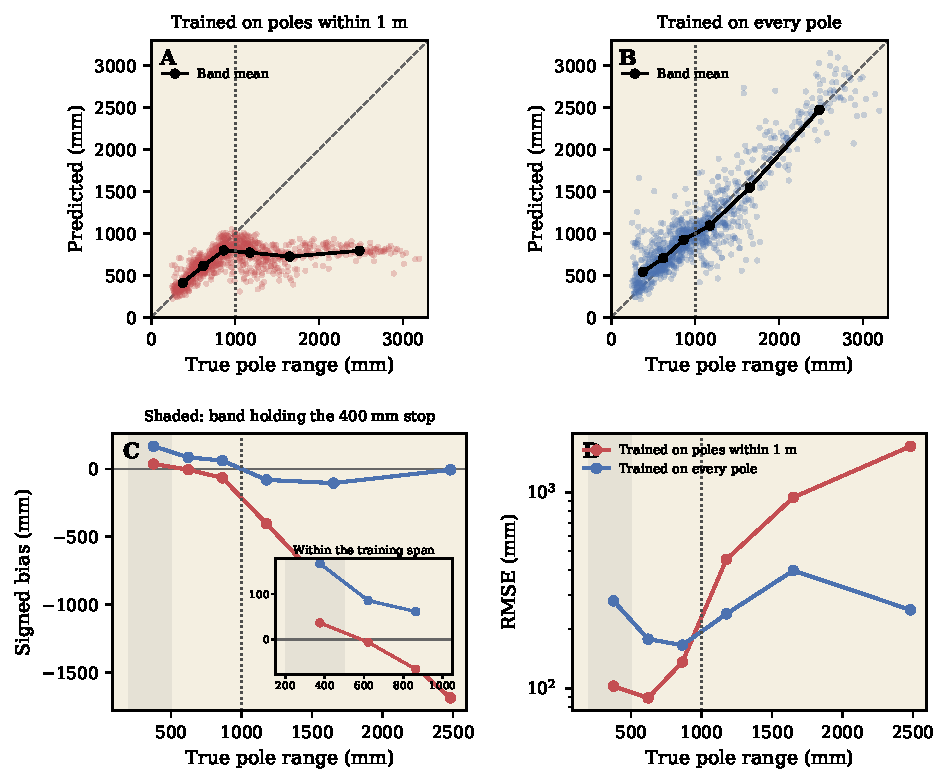
\includegraphics[width=\textwidth]{fig_pole_range_cap}
	\caption{Why the pole-range head is trained only on poles within $1$\,m. Two models differing in one setting: the range span that head is trained on. Both are four-fold quadrant cross-validations over the same $2775$ echoes, so every pole echo is scored once by a model that did not see it. (A) Predictions of the deployed setting, trained on poles within $1$\,m. Past that span it answers about the same distance whatever the true range. (B) Predictions of a model trained on every pole echo, out to $3196$\,mm, which tracks the true range throughout. Black lines are band means; the dotted vertical line marks the $1$\,m training limit. (C) Signed bias against range for both, with an inset over the training span, and (D) the same as RMSE on a logarithmic axis. The shaded strip in (C) and (D) is the band containing the $400$\,mm stop of Experiment 1, which fires on this head's output. Training on every pole echo buys accurate ranging past a metre, at the cost of a close-range bias that grows from $+36$ to $+167$\,mm, in the direction that makes the robot stop nearer than intended.}
	\label{fig:pole-range-cap}
\end{figure}


\end{document}

% =====================================================================
% RETIRED FROM THE INTRODUCTION (2026-06-20 refocus).
% Pulled out of the Introduction when it was refocused around the
% noisy-but-task-usable inverse model and two robot tasks. The
% vicarious-learning framing now belongs in the Discussion (briefer than
% below). Kept here verbatim for salvage; the "vision-as-internal-model
% / planning" argument (Mugan2020, Bennett2023) is the unique content to
% relocate.
%
% --- former Par 6 (vicarious-learning introduction) ---
% \cnote[N]{We should review this paragraph to ensure we introduce vicarious learning in a good way}
% The overlap in feature encoding across modalities also gives rise to a second opportunity. Sensory modalities differ not only in feature accessibility but also in how richly they support internal modeling of the environment. Vision is particularly well suited to this role. Its long operating range gives advance information about distal events, a property argued to have underwritten the evolution of planning and prospective cognition in land vertebrates \citep{Mugan2020,Bennett2023}. We do not have direct evidence that bats build internal spatial representations from vision specifically, but if any modality supports such a representation in this clade, vision is the most plausible candidate. \cnote[x]{Perhaps we can draw on data from rodents and navigation here to suggest that some animals related to bats are capable of internal modeling. We might want to look at the Bennett2023 book. He might list some evidence} A bat with a visual representation of an environment and an inverse model for features available to both sonar and vision could engage in offline rehearsal of behaviors that will later be deployed by sonar alone. In other words, an inverse model for features shared across sonar and vision could support \emph{cross-modal vicarious learning}, i.e., training a behavior through one modality and deploying it through another. \cnote[5]{We should probably add some more arguments for the existence of internal models supported by vision.} Cross-modal vicarious learning would specifically benefit sensory modalities with low informational throughput that are ill-suited to build a coherent environmental representation, such as whisking, sonar, or tactile sensing. Effectively, the representation built using the richer sensory modality (e.g., vision) can be used to train the animal in its use of the more proximate sense.
%
% --- former Par 9 vicarious half + inverse-scope-asymmetry block ---
% Second, we demonstrate cross-modal vicarious learning. Assuming the bat has a visual model of the environment, it can use offline training to perform a spatial task in an environment it has not explored acoustically. The inverse model for this demonstration is therefore trained on echoes collected across a range of arena layouts, again using overhead-camera-derived labels, so that it can support sonar reconstruction of environments the agent has not yet encountered acoustically. We demonstrate this by training the robot to follow a prespecified path through the environment. The asymmetry in inverse-model scope between the two demonstrations mirrors the demands of the two operations. Direct learning calls for a specialized inverse fitted to the operational environment, whereas vicarious learning calls for a general inverse capable of supporting offline rehearsal in counterfactual settings.
% \cnote[N]{In theory, the inverse model for the direct learning task does not have to generalize to new unvisited environments. For the vicarious learning, it has to. However, it seems a bit overkill to train an inverse model on a specific environment for the direct learning only. Perhaps, we don't mention this point here and just mention in the discussion that the inverse model requirement is less stringent for the direct learning?}



%
%Sonar can support the classification of complex natural scenes and objects. Echolocating bats discriminate plant species and other extended targets from the statistics of their echoes \citep{Yovel2009,Yovel2011}, and biomimetic sonar systems reproduce comparable abilities: recognizing places from echo signatures \citep{Vanderelst2016}, detecting passageways in dense foliage \citep{Wang2022}, and retaining, under an efficient encoding, enough spectrotemporal information to match bats across a range of discrimination tasks \citep{Achutha2021}. In one such system, the labels are supplied cross-modally by a camera that teaches an echo classifier which views contain a passageway \citep{Wang2022}, the same supervisory arrangement we adopt here. These studies establish that task-relevant features are physically present in sonar echoes and can be extracted, in some cases under exactly the cross-modal supervision the framework requires. They stop short, however, of showing that such features are used to drive behavior. Where bat-like sonar has controlled an autonomous robot, the behavior relied on echo range and direction rather than on the learned classification, which was demonstrated separately \citep{Eliakim2018}. To the best of our knowledge, it has not been shown that sonar and vision together can be used to learn a feature-based inverse model whose output is sufficient to complete a spatial task.
% =====================================================================
